\documentclass[singelsided,12pt]{mythesis} %this is the mythesis.cls file
% twoside,openright,versioninfo

% Consider:
% \newcommand{\ie}{i.\,e.}
% \newcommand{\Ie}{I.\,e.}
% \newcommand{\eg}{e.\,g.}
% \newcommand{\Eg}{E.\,g.}
\usepackage{graphicx}
\usepackage{amsmath}
\usepackage{booktabs}
\usepackage{pdfpages} % new addition
\usepackage{xparse}
\usepackage{float}
\usepackage{setspace} % new addition
\usepackage[export]{adjustbox}
\usepackage{wrapfig}

%\usepackage{tikz}


\usepackage{geometry} % new addition 
 \geometry{
 a4paper,
 total={210mm,297mm},
 left=35mm,
 right=20mm,
 top=20mm,
 bottom=20mm,
 }


 \usepackage{caption}
\DeclareCaptionLabelFormat{onlyname}{#1}
\captionsetup{labelformat=onlyname,labelsep=period}
\usepackage{sidecap}

\captionsetup[figure]{name={}}
\sidecaptionvpos{figure}{c}

\renewcommand*{\familydefault}{\sfdefault} %% I changed the font
\usepackage{helvet}

\usepackage{geometry} %  I took this from Adams I think it is the right margins
 \geometry{
 a4paper,
 total={210mm,297mm},
 left=35mm,
 right=20mm,
 top=20mm,
 bottom=20mm,
 }


%You might need to load other packages here...

%% Symbols
% unresolved:
\newcommand{\ud}{\mathrm{d}}
\newcommand{\drel}{\ensuremath{r_{\mathrm{rel}}}}
\newcommand{\nmax}{\ensuremath{n_\mathrm{max}}}

\usepackage{natbib}

%Information for the title page
%Some of this is hard coded in mythesis.cls but you can over write if you need to

\title{Predator-prey interactions across scale and dimensionality}
%
\author{Kevin Healy}
%
\month{\textsc{May}} \year{2015}
\previousdegrees{B.Sc., Trinity College Dublin, 2011\\%
}
\degreetitle{Doctor of Philosophy}
\institution{Trinity College Dublin}
\school{School of Natural Sciences}
\department{Zoology}

%End of preamble.

\begin{document}


% \fontfamily{qag}\selectfont

\maketitle %puts in your title

\chapter*{Declaration}
I declare that this thesis has not been submitted as an exercise for a degree at this or any other university and it is, unless otherwise referenced, entirely my own work.
I agree to deposit this thesis in the University's open access institutional repository or allow the library to do so on my behalf, subject to Irish Copyright Legislation and Trinity College Library conditions of use and acknowledgement.
\\
\\
\\
Kevin Healy


\vspace{10 mm}

\chapter*{Summary}
\chaptermark{Summary}
\addcontentsline{toc}{chapter}{Summary}

Predator-prey interactions are an important evolutionary driver of species' form and diversity, and are a central component of ecosystem structure. However, the context dependent nature of these interactions, as reflected by the diversity of species involved, means that understanding them at a fundamental level is required for better and more general ecological predictions. In this thesis I explore the role of two fundamental components of predator-prey interactions: the body size of both predators and their prey; and the dimensionality of the interactions between them. I investigate the fundamental role of body size and habitat dimensionality across three chapters that represent stand-alone publications consisting of: the role of body size on the ability of species to perceive the temporal dimension of their environment; the role of habitat dimensionality and other traits relating to predation pressure on life history evolution; and the role of habitat dimensionality on the evolution of venom in snakes. Throughout my thesis I use comparative approaches to show that both habitat dimensionality and body size are key components that determine the mechanics of predator-prey interactions and hence ecological and evolutionary systems as a whole.

%%% Local Variables:
%%% TeX-master: "thesis"
%%% TeX-PDF-mode: t
%%% End:
 %inputs abstract.tex
\chapter*{Preface} %the * removes the numbers
\addcontentsline{toc}{chapter}{Preface}

Several chapters from my thesis have been published elsewhere:

\lettherebespace
\textsc{chapter one} has been previously published as:
%
\begin{previouspaper}
  \textbf{Healy K.,} McNally, L., Ruxton, G.D., Cooper, N., Jackson, A.L. 2013. Metabolic rate and body size are linked with perception of temporal information. \textit{Animal Behaviour}, 86, 685-696.
\end{previouspaper}
 
As lead author I was involved with the initial conception of the paper, I collected the data, designed and ran the analysis and wrote the manuscript.


\lettherebespace
\lettherebespace
\textsc{chapter two} has been previously published as:
%
\begin{previouspaper}
  \textbf{Healy K.,} Guillerme, T., Finlay, S., Kane, A., Kelly, S.B.A., McClean, D., Kelly, D.J., Donohue, I. Jackson, A.L., Cooper, N. 2014. Ecology and mode-of-life explain lifespan variation in birds and mammals. \textit{Proc. R. Soc. B}, 281, 20140298 .
\end{previouspaper}

As lead author I was involved with the initial conception of the paper, collection and management of the data, designing and running the analysis and writing the manuscript.

\begin{previouspaper}
  \textbf{Healy K.} 2015. Eusociality but not fossoriality drives longevity in small mammals. \textit{Proc. R. Soc. B}, 282, 20142917 .
\end{previouspaper}

I replied to the comment by \cite{williams2015ecology} on the paper above were they show eusociality is an important factor to consider for lifespan evolution in fossorial mammals. I carried out additional analysis showing that including the error associated with phylogeny construction further strengthens the association between of eusociality and increased lifespan.


%Here I explain what I did for this paper, and what the other coauthors did. Can just repeat this for each chapter if all are published already or in prep. Basically for anything you do with other people.
%%%%%%%%%%%%%%%%%%%%%%%%%%%%%%%%%%%%%%%%%%%%% %inputs preface.tex
\allcontents %tells it to make a table of contents with figure and table lists too
% There is currently a problem with spacing somewhere so that Table of
% Contents, List of Tables, and List of Figures have the wrong amount
% of space.  Others are OK though...
\chapter*{Acknowledgements}
\addcontentsline{toc}{chapter}{Acknowledgements}


For the last eight years Trinity has been my academic home in the big smoke where I have been lucky enough to have met and received the help and kindness of so many people, without which I certainly would not have gotten to the brink of the big Dr. For even allowing me into Zoology I would like to thank both Prof. Trevor Hodkinson and Dr John Rochford who helped me transfer to Zoology in my first year (the second best decision of my life so far), saving me from the terrible clutches of Physics. Once safe within the interior of the Zoology Building I got to be part of many inspiring lectures including from Prof. Celia Holland who I thank in particular for inspiring me to chase my interests as an undergraduate and for guiding me so patiently during my final year thesis. A big thank you to my supervisor Dr Andrew Jackson who not only gave me the opportunity to continue to do science in Trinity but gave me the full license to do the science that put a smile on my face for the last four years and for providing so much support throughout. I have the Jackson lab to also thank for making my PhD so enjoyable, Luke McNally and Mafalda Viana helped immensely in guiding me through the art of science before back-up in the form of Adam Kane and his endless depravity for puns helped keep my heady morning cynicism at bay. The office would also certainly have been a lesser place without the Cooper due of Sive Finlay and Thomas Guillerme who along with Dr Natalie Cooper brought so much to the department both academically and personally. The door to our office was usually open and for good reason, the input, support and chin-wags from Deirdre McClean, Se{\'a}n Kelly and the whole cast of NERD club has always been a welcome respite to when research started to feel like real work.  

I would like to thank all my family who have always supported my absurd decision to choose science as a career and who have always been there through both the good and bad. Finally a very special thank you to Emily Keely who not only put up with my late nights behind a screen but made my time in Trinity so special.


%%% Local Variables:
%%% TeX-master: "thesis.tex"
%%% TeX-PDF-mode: t
%%% End:
 %inputs acknowledgements.tex
\cleardoublepage
\mainbody

\chapter{General Introduction}
\label{chap:introduction}%Note this label will be used to refer to the chapter throughout. So if you change the order of chapters it still knows this one is this file, but can call it chapter 1 or 2 or whatever depending on the order. S oti's better than calling it chapter 1.

%\begin{quoteshrink}
 % ``I can mention many moments that were unforgettable and revelatory. But the most single revelatory three minutes was the first time I put on scuba gear and dived on a coral reef. It's just the unbelievable fact that you can move in three dimensions.''
%  \hfill{David Attenborough}
%\end{quoteshrink}

\noindent
The ability to both obtain and avoid becoming food is one of the primary selection pressures driving animal evolution. Predator-prey interactions not only shapes the species directly involved in these interactions but also form the fundamental building blocks of ecosystem structure making them key to our understanding of biological systems as a whole \citep{pimm1984complexity,cohen1990community}. However while these interactions are ubiquitous across diverse ecosystems each predator-prey interaction plays out within its own specific context. For example, even if hunting the same prey one predator may rely on venom to incapacitate prey while another may rely on a strategy of high performance aerobatics to meet the same ends. However amongst these context dependencies commonalities arise across which provide a clear approach to understand how these interactions emerge and effect they have on the systems in which they are embedded.


While the arms race between predators and their prey plays out across a diversity of forms, all players must abide to the fundamental constraints imposed by physics. For example biomechanical and physiological limitations result in flying species remaining relatively small \citep{chatterjee2007aerodynamics,dudley2002mechanisms} while the largest species are invariably found in the oceans \citep{heim2015cope}. It is within these boundaries of physics that evolution trades off between the benefits of investing in traits relating to that species predator-prey interactions and the energetic costs associated with developing such traits. One common way for these trades-offs to present themselves is through there link with both body size and interaction dimensionality.


Since Kleiber fist demonstrated the link between the rate of energy utilised by an animal and its size \citep{kleiber1947body} ecology has utilised this correlation to understand a range of biological processes and principles (refs). More recent formulations have attempted to use the fractal structure of physiological systems as a first principle approach to unify many aspect of biology such as physiology, behaviour and ecology \citep{west1997general,brown2004}. While heated debate surrounded the exact nature of this scaling and the fundamental basis that underpinning it (refs summing this up), this scaling relationship has become one of the most useful proxies to many elements of biology, including predator-prey interactions \citep{brown2004}. While body size and metabolic rate have featured as the main element of this drive to find fundamental elements within biological complexity the dimensionality of the arena these interaction play out in has more recently been found to play a key role.


Similar to the formalisation of metabolic theory in the mid 90's the role of habitat complexity in biology has its roots in utilising the mathematics of fractals in order to explain macroecological patterns. \cite{morse1985fractal} was the first to utilise this geometry to describe how the dimensionality of vegetation can determine arthropod community densities through the available habitat structure created by space filling properties of the plants. The the effects of habitat dimensionality was further explored in particular in primary consumers and their prey etc (see Pawar and my old thesis for refs). More recently habitat dimensionality has been re-framed as the dimensionality of the interaction between predator and prey \citep{pawar2012dimensionality}. This framework has allowed dimensionality to be explored across larger groups and foraging strategies and extended the predictive ability based on body mass scaling through the finding that high dimensional interactions have steeper scaling with body mass then expected from standard theory. It also opens up the importance of the role of sensory ecology within such interactions, in particular as such sensory systems have shown different scaling in comparison to that predicted from metabolic theory. %maybe need to include something about that in time perception model.


This thesis draws on how these two fundamental pillars of biological structure affect predator-prey interactions across the range of contexts these interactions take place. By using comparative methods I will focus on three areas; how do species sample and perceive the temporal dimension; the role of habitat dimensionality in prey species life history; and the role of habitat dimensionality in the evolution of predatory traits. By understanding the forces shaping species within the dimensions of their habitats we can gain deeper understanding of the mechanics of predator-prey interactions as a whole.


\section{\uppercase{R}esearch outline}


\textbf{Chapter 2: Body size, metabolic rate and visual temporal perception in vertebrates.}

 All organisms must perceive the temporal dimension of their environment. This is particularly true of predators and their prey that need to accurately track and predict their adversaries' motion. Here I collate data on a measure of visual temporal perception called critical flicker fusion to test whether species that are predicted to be more maneuverable can perceive events at finer scales. I show that, as expected, small species with high metabolic rates have the fastest perception of time. This has important consequences for the ability of predators to capture their prey and I discuss some examples of adaptations in predator species that potentially mitigate against this general trend. 


\textbf{Chapter 3: Ecology and mode-of-life explain lifespan variation in birds and mammals.}

Maximum lifespan varies strongly with body mass yet many species live far longer than expected given their size. This may reflect interspecific variation in extrinsic mortality, as life-history theory predicts investment in long-term survival when extrinsic mortality is reduced. Here, I investigate how ecological and mode-of-life traits that are predicted to reduce extrinsic mortality influence lifespan across mammals and birds. I show that species associated with high dimensional habitats, namely arboreal and volant species, show longer lifespan than expected for their body size. I discuss how habitat dimensionality may affect exposure of prey to predation pressures and the role of other ecological traits including fossoriality, eusociality, and activity patterns.


\textbf{Chapter 4: Habitat dimensionality and a diet of eggs; the evolution of venom loss in snakes.}

Despite the obvious advantages of possessing venom there is little explanation for variation in the volume and toxicity of venom in snakes. This is particularly apparent in species that partially or fully lose the capacity to produce venom such as demonstrated in sea snake species. As venom is primarily used for capturing prey I test whether fundamental factors, including habitat dimensionality and diet, affect the amount of venom produced within a species through their influence of encounter rates and prey toxicity resistance. By collating data on venom toxicity (LD50), diets, body size, environment dimensionality and both maximum and minimum venom volumes comprising of over 75 species, I show that species found in high dimensional environments or that have egg-based diets produce less venom than their counterparts. I also demonstrate the prey-specific nature of venom toxicity using phylogenetic distance between diet species and LD50 model species as a test. I discuses the possible mechanisms and the implications of these results in relation to both evolution of venom and costly predatory traits in general.

%
%
Finally, in \chapref{conclusions}, I close with a discussion of the
limitations of the methods used in the thesis, and suggest some future
directions.

\section{\uppercase{A}dditional work}
In addition to the chapters enclosed in this thesis, I have also been involved in the following research during my studies:\\




\bibliographystyle{PLoS-Biology}
\bibliography{bibfile}

 %This is a ch1-introduction.tex file with contents of intro chapter
\chapter[Temporal perception, body size and metabolic rate]{Metabolic rate and body size are linked with perception of temporal information}
\label{chap:CFF}


\begin{figure}[h]
  \centering
  \includegraphics[width=.45\textwidth]{ch2-time/eyepic.png}
\end{figure}

\begin{quoteshrink}
  ``Time is an illusion. Lunchtime doubly so.''

\hfill{Douglas Adams}
\end{quoteshrink}

%%And suddenly I realised that I was no longer driving the car consciously. I was driving it by a %%kind of instinct, only I was in a different dimension.
%% Ayrton Senna


\begin{abstract}
Body size and metabolic rate both fundamentally constrain how species interact with their environment. While many mechanisms leading to these constraints have been explored, their effects on the resolution at which temporal information is perceived have been largely overlooked. The visual system acts as a gateway to the dynamic environment and the relative resolution at which organisms are able to acquire and process visual information is likely to restrict their ability to interact with events around them. As both smaller size and higher metabolic rates should facilitate rapid behavioural responses, these traits would be predicted to favour perception of temporal change over finer timescales. Using critical flicker fusion frequency, the lowest frequency of flashing at which a flickering light source is perceived as constant, as a measure of the maximum rate of temporal information processing in the visual system, I find support for this hypothesis across a wide range of vertebrates. These results have implications for the evolution of signalling systems and predator-prey interactions, and, combined with the strong influence that both body mass and metabolism have on a species' ecological niche, suggest that time perception may constitute an important and overlooked dimension of niche differentiation.
\end{abstract}

\section{Introduction}

All biological systems, from organisms to ecosystems, are shaped by universal constraints. For example, body size and metabolic rate are both known to be important determinants of organism biology, influencing life history, energetics and behaviour \citep{brown2004, woodward2005, sibly2012metabolic}. More recently the fundamental role of sensory biology in ecological interactions has gained attention, such as in the limitations of target identification \citep{tosh2010modelling} and the scaling allometry of sensory organs \citep{howland2004allometry,cronin2005role,garamszegi2002coevolving,kiltie2000scaling}. The limitations such sensory systems are constrained by can determine ecological interactions through, for example, predation and mate selection where the abilities of the parties involved to capture, escape or be seduced is dependent on how they perceive their environment (Fig. 1; \citealt{cronin2005role,clark2012field,hornstein2000sexual,stevens2007predator}). While the ability and importance of an organism to perceive the spatial dimensions of its environments are relatively well studied \citep{cronin2005role,clark2012field}, how they perceive the 4\textsuperscript{th} dimension, time, is less well known.

As the environment is fundamentally dynamic in nature, the ability to integrate information over a time period is a necessity for any organism. Furthermore, the ability to integrate information over shorter timescales, that is, at higher resolutions, is a direct limitation on the degree to which it can interact with the environment itself. From an evolutionary perspective this leads to a trade-off between the demand for information at high temporal resolutions and the costs of its acquisition given the energetic demands associated with increased rates of neural processing in the visual system \citep{laughlin2001energy}. This trade-off is likely to be shaped by various ecological (e.g. mode of predation) and environmental factors (e.g. light levels) as well as intrinsic factors (e.g. morphology) that will ultimately shape an organism's optimal temporal resolution for sensory perception \citep{autrum1958electrophysiological}.


\begin{figure}[p]
  \centering
  \includegraphics[width=.95\textwidth]{ch2-time/Figure_1.jpg}
  \caption[ ]{Figure 1. The ability of an organism to track a moving object depends on the time integral over which the individual can obtain its information. This is determined by its ability to resolve temporal information. In cases where an animal, such as a ground squirrel, displays complex movement (a), conspecifics may perceive the individual as moving according to a first-order integral of its actual movement owing to its high temporal resolution abilities (b). However a species with lower temporal resolution abilities, such as a short-eared owl, may perceive the motion as an even higher order derivative of the actual motion, meaning information of prey motion at finer temporal scales is not available to it (c).}
  \label{fig:Figure 1.}
\end{figure}


This ability to perceive and react to a dynamic environment is also likely to be an important behavioural and ecological trait. Ecologically, interaction strengths can be affected by the ability to identify and track fast-moving objects such as prey or mates (Fig. 1; \citealt{land1974chasing, fritsches2005warm}). The necessity of this ability to perceive one's environs accurately is perhaps best demonstrated in cases where temporal resolution is too coarse to allow the observer to follow the motion of a moving target accurately. A stark demonstration of this can be seen in the tiger beetle, \textit{Cicindela hudsoni}, which, owing to the relatively low temporal resolution of its visual system, must take a stop-start approach in order to recalibrate the position of its prey when hunting \citep{gilbert1997visual}. In humans, the limitations of our temporal perception are apparent when tracking fast-moving objects such as the curving trajectory of a ball in soccer \citep{dessing2010bending} and baseball \citep{bahill2004rising} and is also directly linked to the perception of the passage of time itself \citep{hagura2012ready}. 

Two intrinsic factors that may shape the costs and benefits of the temporal resolution of the sensory system, in particular with respect to their effects on an individual's ability to interact with the environment on short timescales, are body size and metabolic rate. As larger body sizes decrease manoeuvrability \citep{heglund1988speed,dudley2002mechanisms,biewener2003animal,sato2007stroke,vogel2008modes,hedrick2011damping,watanabe2012slowest} and higher metabolic rates increase both manoeuvrability and the physiological ability to process information \citep{li2008optimal,franz2002temperature}, smaller organisms and those with higher metabolic rates would be predicted to perceive temporal change on finer timescales.

To quantify the temporal perceptual abilities of a range of species I take advantage of the all-or-nothing nature of neural firing in the visual system. Owing to this binary firing, temporal resolution must be encoded in terms of discrete units, as biological visual systems must discretise the continuous-time and continuous-space information reaching the retina and then integrate this information over some time period. This "integration time" of visual systems can be quantified using the critical flicker fusion frequency (CFF): the lowest frequency of flashing at which a flickering light source is perceived as constant \citep{d1998can,schwartz2010visual}. As light intensity can increase the number of flashes that can be observed per second, the maximum CFF value, as measured in a response curve of CFF against light intensity \citep{ferry1892persistence,porter1902contributions}, can be used as a proxy for the temporal resolution of the sensory system.

Here I use maximum CFF to compare the temporal resolution of the visual system in a wide range of vertebrate species including representatives from Mammalia, Reptilia, Aves, Amphibia, Elasmobranchii and Actinopterygii. Using phylogenetic comparative methods and controlling for the light levels each species typically experiences, I test whether the temporal resolution of the sensory system increases with mass-specific metabolic rate and decreases with body mass.

\section{Methods}
\subsection{Data Collection}
To test the prediction that CFF increases with mass-specific metabolic rate and decreases with body size (when controlling for light levels), data on maximum CFF values in vertebrate species was collated from the literature (Table \ref{tbl:Table 1.}). Only values from studies that measured CFF using either behavioural or electroretinogram (ERG) procedures were included. In behavioural studies, CFF is measured through conditional training with the subject trained to respond to a change in its perception of a flashing light \citep{d1998can,rubene2010presence}. For example, \cite{lisney2011behavioural} conducted behavioural tests in domestic chickens, \textit{Gallus gallus}, using choice experiments with flickering and non-flickering stimuli windows with choice of the correct stimulus rewarded with food. This is repeated over a range of light intensities and flicker frequencies until individuals can no longer distinguish between the stimuli. In ERG studies, a direct measurement of the electrical response in the retina in reaction to a flashing light source is used as a measure of CFF \citep{d1998can,schwartz2010visual}. As there may be further processing of temporal information after it reaches the retina that may cause behavioural studies to measure lower CFF values \citep{d1998can}, the experimental procedure used to measure CFF was included as a candidate covariate. 
%We also noted whether each study was a reliable measure of the maximum possible CFF. As maximum CFF is a function of many variables, such as light intensity, and not all studies reported a sufficient range of intensities, their reported CFF may not be the "true maximum" possible. To ensure this did not affect our results we ran an additional analysis that included a term based on this assessment as a categorical covariate as part of our sensitivity analyses (see Appendix).
%changethe end of that to less weak response

Mean body mass (g) published in the literature and in databases including FishBase \citep{froese2012fishbase} and Animal Diversity Web \citep{myers2006animal} was collected for each species as the measure of body size. For metabolic rates mass-specific resting metabolic rate as measured by oxygen consumption through ventilation  was used were the subjects were fasted prior to the measurement. These values were converted to W/g using the conversion of 20 J/ml of oxygen consumption \citep{makarieva2008mean} to allow comparison among species. For ram-ventilation species (which require constant movement to force fluid over the respiratory organs), such as sharks and tuna, the resting metabolic rate was taken as the fitted line of oxygen consumption with swimming speed extrapolated to the intercept (swimming speed = 0 m/s; Table 1.). To account for the possible effect of metabolic rate measured at different temperatures in ectothermic species, metabolic rate values were corrected to 20 $^{\circ}$C using Q10 values, i.e. the fold change in metabolic rate over a temperature change of 10 $^{\circ}$C, for reptiles, amphibians and fish \citep{white2006scaling}. These corrections gave values of temperature-corrected mass-specific resting metabolic rates (qWg), for each species. Although body mass and mass-specific metabolic rate are expected to be correlated according to an exponent of 0.25 \citep{brown2004, sibly2012metabolic} (Brown et al., 2004 and Sibly et al., 2012), both terms were included as recommended by \cite{freckleton2009seven} instead of using residuals from a regression of body mass against mass-specific metabolic rate.

As there is a trade-off between sensitivity and movement perception owing to the requirement of longer integration times in low light conditions \citep{tansley1965vision}, as is seen in the different light response dynamics of rods and cones \citep{rubene2010presence}, light levels was included in the analyses as a categorical variable based on the light conditions experienced by the species during normal activity (i.e. foraging). Species were categorized as inhabiting either high or low light conditions with diurnal terrestrial and nonturbid aquatic species coded as inhabiting high light level environments and nocturnal species coded as inhabiting low light levels. As the light levels of species that inhabit turbid waters are typically orders of magnitude lower than typical daylight levels (40-1000 lx; \citealt{ali1985vision,palmer2010art,kreysing2012photonic}) and the harp seal, Pagophilus groenlandicus, regularly forages at depths greater than 200m \citep{folkow2004distribution} where light levels are comparable to nocturnal light levels (Palmer and Grant 2010), these species were categorized as inhabiting low light level environments.


\begin{figure}[h!]
  \centering
  \includegraphics[width=.95\textwidth]{ch2-time/phylofig.pdf}
  \caption[ ]{Figure 2. Phylogeny of species used in analysis. Scale bar represents million of years. See appendix A for divergence times.}
  \label{fig:Figure 2.}
\end{figure}


To correct for the phylogenetic nonindependence of species within the analysis a composite tree was constructed using published molecular phylogenies and divergence times from various sources (\cite{schoch1985preliminary,janossy2011pleistocene,mercer2003effects,hedges2006timetree,wiens2006does,benton2007paleontological,murphy2007using,brown2008strong,li2008optimal,naro2008evolutionary,albert2009effect,lim2010phylogeny,little2010evolutionary,perelman2011molecular}; see Appendix A and Figure 2). In instances were a divergence time was not available for two species a conservatively estimated date of first appearance was used as the divergence time taken from the Paleobiology Database \citep{alroy2008phanerozoic}.


As ectotherm metabolic rates vary with temperature, a sensitivity analysis to test the effect of the temperature to which qWg was corrected was performed by rerunning the main analysis with qWg corrected to both 5 $^{\circ}$C and 35 $^{\circ}$C (see Appendix A). A supplemental analysis on a more restricted data set for species with available brain mass data was also carried out to test for any possible effects of sensory tissue on maximum CFF values (see Appendix A).

In total data on maximum CFF, body mass, qWg and light environments for 34 species across the vertebrate classes Elasmobranchii, Actinopterygii, Aves, Amphibia, Reptilia and Mammalia was collected, with further data on brain mass for 28 of these species (Table 1).


\begin{table}[!Hp]
  \caption[ ]{Table 1. Data used in the analysis including, maximum critical flicker fusion (CFF), Mass in grams (Mg), mass specific resting metabolic rate corrected to 20 $^{\circ}$C in ectoterms (qWg), Brain Mass in grams, Light levels (L = low, H = High)}
  \label{tbl:Table 1.}
  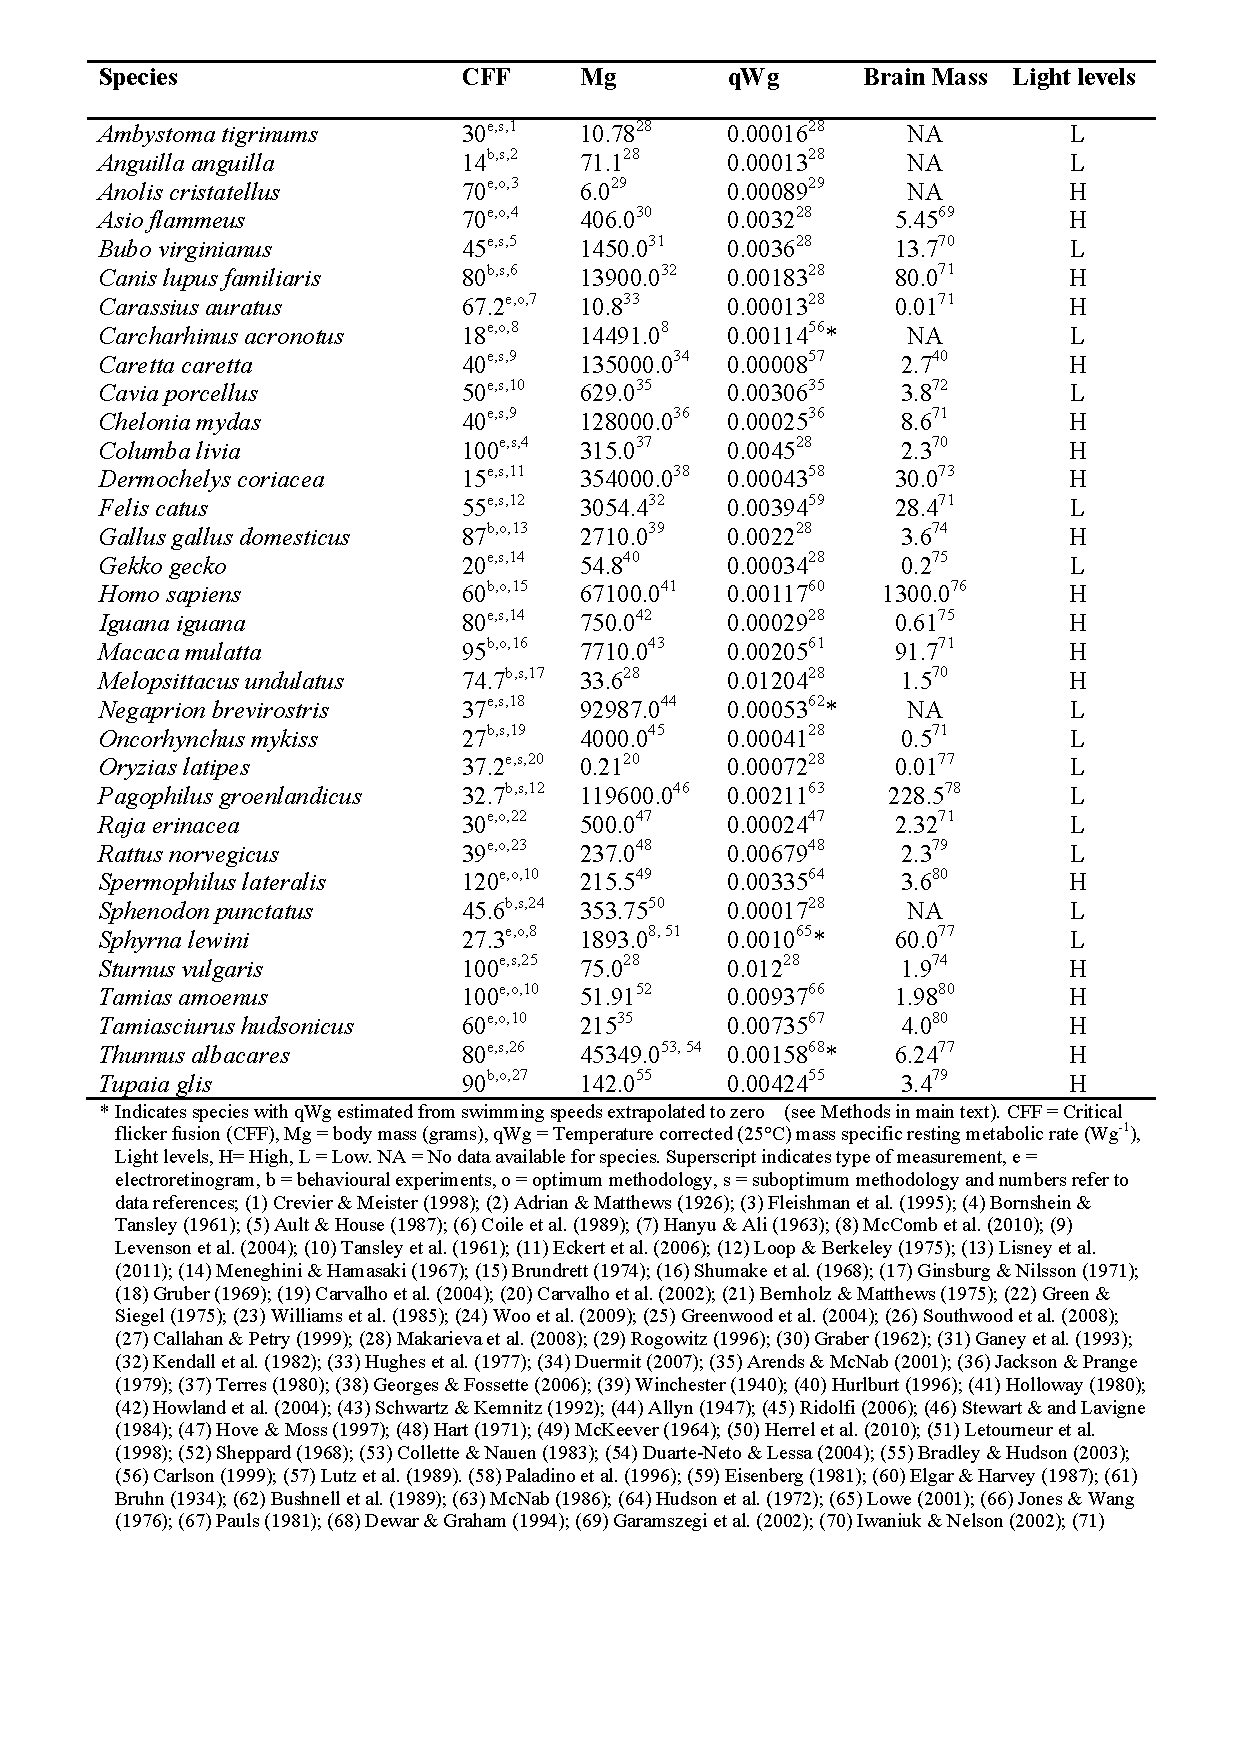
\includegraphics[width=1.0\linewidth]{ch2-time/Table_1}
\end{table}


\subsection{Statistical Analyses}
To test the hypothesis that small species with high metabolic rates show the highest CFF values, I used a phylogenetic generalized least-squared approach (PGLS) using the caper package \citep{orme2011caper} in R version 2.14.2 \citep{RCran}. This approach allows for nonindependence in the data caused by species' phylogenetic relationships to be accounted for by incorporating it through the error term structure \citep{pagel1999inferring,rohlf2001comparative}. This error term consists of a matrix of expected trait covariances calculated using the maximum likelihood estimate of lambda ($\lambda$), a multiplier of the off-diagonal elements of a phylogenetic variance-covariance matrix that best fits the data. When the data are structured according to a Brownian motion of trait evolution, lambda = 1, whereas when the data have no phylogenetic dependency, then lambda = 0 \citep{pagel1999inferring}.


The analysis consists of PGLS models with maximum CFF as the response variable, and all combinations of the following explanatory variables: body mass, qWg, light level (high, low) and experimental procedure (ERG, behavioural) with brain mass included in the sensitivity analysis (see Appendix A.2.2).
%, with Akaike's information criterion (AIC) used to select the minimum adequate model \citep{burnham2002model}.

%\newpage

\section{Results}
In the main analysis body mass had a negative effect on the temporal resolution of the sensory system (Table 2, Figure 3a), while metabolic rate, after correcting for mass and temperature, was positively associated with CFF (Table 2, Figure 3b) and low environmental light levels were associated with an overall reduction in CFF (Table 2, Figure 3). Phylogeny was found to have a minimal effect on the resulting models ($\lambda$ = 0, Table 2) and experimental type was not correlated with CFF (Table 2). Thus, according to our model, small animals with high mass-specific metabolic rates in high light environments possessed the highest maximum CFF and hence greatest ability to perceive temporally dynamic visual information. Conversely, large animals with low mass-specific metabolic rates in low light environments had the lowest CFF.


\begin{table}[h!]
  \centering
    \caption[ ]{Table 2. Coefficients of the model with all factors included. Mg = body mass (grams), qWg = Temperature corrected mass-specific resting metabolic rate Wg-1, Light.l (low) = effect of low light levels on CFF in comparison to high light levels, exp = effect of experimental type (ERG = electroretinogram) in comparison to behaviour based CFF measures.}

\begin{tabular}{*5l}    \toprule
\emph{Variable} & \emph{Estimate} & \emph{S.E} & \emph{t-value}&  \emph{P-value}\\\midrule
Intercept    & 141.48  & 15.15  & 9.34  &  {\ensuremath{4^{-10}}}\\ 
Mg & -4.40 & 2.01 & -2.18 & 0.038\\
qWg & 16.89 & 4.31 & 3.92 & {\ensuremath{5^{-4}}}\\
Light levels (low) & -37.74 & 5.94 & -6.36 & {\ensuremath{7^{-7}}}\\
Measurement type (exp) & -3.66 & 6.24 & -0.59 & 0.56\\
Data quality (high) & -3.86 & 6.14 & -0.63 & 0.53\\
 &  & & & \\
 & Mode & Lower 95\% C.I & Upper 95\% C.I\\ 
Lambda  (Low) & 0 & 0 & 0.34 &\\
&  &  &  &{\ensuremath{R^2}= 0.69}\\\bottomrule
 \hline
\end{tabular}
  \label{tbl:Table 2.}
\end{table}


These results were robust to the sensitivity analysis on both the temperature used to correct ectotherms qWg (taken as 20 $^{\circ}$C in the main models above; see Methods) showing the same trends as found in the main analysis (Appendix A.2.1). Including brain mass in a restricted data set of 28 species for which brain mass was available did not change the effect of the explanatory variables light levels, qWg and body mass on maximum CFF ( Appendix A.2.2).


\begin{figure}[h!]
  \centering
  \includegraphics[width=.95\textwidth]{ch2-time/Figure_2}
  \caption[ ]{Figure 3. The effect of  log$_10$ body mass, light levels and log$_10$ temperature corrected mass-specific resting metabolic rate (qWg) on critical flicker fusion frequency (CFF). The minimal adequate model (Results) indicates CFF increases with log$_10$ qWg but decreases with body mass. Low light levels (blue) are associated with low CFF values in comparison to high light levels (red).}
  \label{fig:Figure 3.}
\end{figure}


\section{Discussion}
Many of the interspecific and intraspecific interactions that shape species' behaviour and ecology rely on the ability of organisms to process high temporal resolution sensory information. These results show that, while there is considerable variability in the ability to resolve temporally dynamic visual information across vertebrates, body mass and metabolic rate act as important general constraints on this ability. This is the first study to indicate a general trend in the ability of vertebrates to resolve temporal information; previous studies have generally focused on specific cases of sensory adaptations \citep{fritsches2005warm} and particular environments \citep{frank1999comparative,frank2012light}, hence focusing on the particular ecological context of each adaptation or environment. These findings illustrate the relationship between both physiology and the effects of body mass on the ability to resolve temporal features of the environment on fine timescales, hence linking sensory adaptations to fundamental constraints and trade-offs imposed on all organisms.


The finding that metabolic rate strongly influences temporal perception extends the known influence metabolism has on organism biology. The rate at which sensory tissue can function is dependent on both the energy available and the tissues temperature. Furthermore, the rate at which neurons can transmit information is dependent on the rate at which proton pumps can re-establish a gradient potential after firing, which in turn is dependent on metabolic rate \citep{laughlin2001energy}. It is unsurprising hence that species which have high metabolisms also benefit from an increased in the rate of sensory system functioning. In contrast species which cannot benefit from the increased rates of sensory firing are likely to reduce investment into such sensory systems, such as the case in the visual system of the deep sea escolar which has one of the lowest temporal perception of any vertabrate \citep{landgren2014visual}. This reduction of investment in temporal perception is likely to partially explain the separate negative affect of body size on temporal perception as larger species in general have decreased manouverability \citep{heglund1988speed,dudley2002mechanisms,biewener2003animal,sato2007stroke,vogel2008modes,hedrick2011damping,watanabe2012slowest} and hence less ability to react to the environment. This idea is supported by research showing that faster and more manoeuvrable fly species have higher temporal resolutions \citep{laughlin1993fast} and that less manoeuvrable species of scavenger crabs display slower response dynamics than deeper living predatory species which are likely to have more active lifestyles \citep{frank2012light}. 


While these findings establish a fundamental scaling between temporal perception, metabolism and body size many species demonstrate physiological adaptations which allow for increase sensory perception despite their size and metabolic rate. For example despite their large size predatory swordfish are capable of a ten-fold increase in their CFF, levels expected of a small endotherm in this model, through specialised heating tissues in thier eyes \citep{fritsches2005warm}. This is achieved through this specialised tissue increasing the temperature, and hence the metabolic rate, in their visual systems allowing them to up-regulating their CFF when hunting \citep{fritsches2005warm}. Similar adaptations are also seen in other species of large, fast-swimming predatory fish \citep{carey1982brain,block1985warm,Wegner15052015} and species of blowfly \citep{tatler2000temperature}. Physiological adaptations for high-resolution motion detection are also found within specific areas of the retina in some flies, commonly referred to as the "love spot", which allow them to identify female flight patterns accurately and thus detect mates \citep{land1974chasing}. 
%However these species are likely to define the exception over the rule, as most species in our analysis fit well to the predict scaling.
%Andrew doesnt like this line its a bit of an unnecassary apology for residuals.

The effects of body size and metabolic rate on temporal resolution and the presence of sensory adaptations also point towards an interesting axis of niche space. Disparity in size and metabolic rate among species within an ecological setting may select for particular sets of adaptations creating a diverse set of sensory systems and interactions. In such a system, species might occupy the same spatial and temporal niche,
%I changed dimension to axis. 
 but could be separated owing to differential responsiveness to environmental signals and cues as a result of having evolved divergent signalling systems along an axis represented by temporal resolution. For example, it seems at least theoretically possible to encode information in high-frequency signals that can be detected by intended receivers such as conspecifics but that are not susceptible to "eavesdropping" by (generally larger) predators. In fact this idea has already been utilized to develop fishing lures which are perceived as flasing lures by the target catch species yet are well camouflaged to unwanted by-catch such as marine turtles \citep{jordan2013linking,crognale2008leatherback}. Ecological systems in which this may be realised include deep-sea systems where visual signalling is an important determinant of the ability of organisms to interact, and where bioluminescence flashing over wide frequency ranges is ubiquitous \citep{haddock2005bioluminescent,widder2010bioluminescence}. Similarly urban lighting may also create such variation in perceptional space for species with possible negative affects on species with high temporal perceptions as the flickering rate of street light may both reduce the advantages such species have over their prey or cause increased stress such as observed in birds species kept in captivity \citep{inger2014potential}. 
%put in bats maybe?


Overall these results show that not only are body size and metabolic rate good proxies for the rate of biological interactions, they are good proxies for the ability to perceive such interactions. While interaction rates are strongly coupled with the spatial dimensionality of the environment and searching rates associated with them \citep{pawar2012dimensionality} the temporal dimension in which an individual resides will also strongly influence its ability to interact with that environment. The generality of these findings suggest that temporal resolution may play a much more important role in sensory ecology than previously indicated, in particular because of its universal effects relating to metbolism and body size. Further investigations into both the underlying mechanisms of these findings and their importance to ecological functioning are needed.


%\bibliographystyle{PLoS-Biology}
%\bibliography{bibfile}


	%This is a ch2-labstudy.tex file with contents of intro chapter etc.
\chapter[Longevity]{Ecology and mode-of-life explain lifespan variation in birds and mammals}
\label{chap:Longevity}


\begin{figure}[h]
  \centering
  \includegraphics[width=.20\textwidth]{ch3-longevity/long.png}
\end{figure}


\begin{quoteshrink}
  ``Achieving life is not the equivalent of avoiding death.''
  
\hfill{Ayn Rand}
\end{quoteshrink}

%%%%%Always keep your smile. That's how I explain my long life. Jeanne Calment



\begin{abstract}
Many species live far longer than expected given their body mass. This may reflect interspecific variation in extrinsic mortality, with species capable of reducing mortality expected to exhibit longer lifespans. One such factor that may strongly influence such extrinsic mortality is habitat dimensionality. As higher dimensional habitats create multiple escape routes from predation, species associated with such environments would be expected to have higher maximum lifespans. Here, I investigate how such traits associated with habitat dimensionality inducing volancy, arboreality and fossoriality, along with other potential traits, including activity patterns and eusociality, influence lifespan across birds and mammals. Using phylogenetic comparative analyses with over 1300 species I show that, over and above the effect of body mass, species associated with high dimensional habitats, through arboreality and the ability to fly, live the longest. Within volant species, lifespan depended upon when (activity patterns), but not where (foraging habitats), species are active. However, the opposite was true for non-volant species, where lifespan correlated positively with both arboreality and whether they were eusocial. These results indicate that dimensionality can affect the ability of prey to escape predation with the resulting affects on species life-history evolution. 

\end{abstract}

\section{Introduction}

Lifespan, or longevity, is a fundamental life-history trait that exhibits considerable variation both within and among species. Maximum lifespan in vertebrates, for example, ranges from up to 211 years in the bowhead whale (Balaena mysticetus;\citep{de2009database}), down to just eight weeks in the pygmy goby (Eviota sigillata; \citep{depczynski2005shortest}). Like most other life-history traits, lifespan varies strongly with body size such that large species tend to live longer than smaller species \citep{lindstedt1981body,promislow1993size,de2007analysis,ricklefs2010life}. However, many species have far longer, or indeed shorter, lives than expected given their body mass (Figure \ref{figure:Figure 1.})). Understanding the mechanisms underlying these deviations from predicted lifespan may reveal the secrets to treating and combating human ageing \citep{ricklefs2010insights,zhang2013comparative}. 

One explanation for species living longer than expected, given their body size, is that low extrinsic mortality (i.e. low risk of death due to external causes such as disease, predation, food shortages  or accidents) will, on average, select for longer lifespans than when extrinsic mortality is high \citep{stearns1992evolution,Williams1957}. This is because when untimely death is more likely, investment in early and frequent reproduction is favoured rather than investment in long-term maintenance and survival. Therefore, species with adaptations that reduce the risks of extrinsic mortality should live longer than expected, given their body mass \citep{partridge1993optimality}. These ideas have led to myriad, taxon-specific hypotheses about traits that may reduce extrinsic mortality and result in increased lifespan \citep{ricklefs2010insights}. However, there is little consensus about the general drivers of increased lifespan across clades.

As predation is one of the main sources of extrinsic mortality, species which possess the ability to reduce it, for example through the use of toxin defences, show increased lifespans \citep{hossie2013species}. One fundamental ecological aspect that would be expected to affect such predation pressures is the dimensionality of the habitat a species lives within. The dimensionality of trophic interactions is a key element in predation pressures where consumption rates scale higher with body mass in high dimensional interactions \citep{pawar2012dimensionality}. While this increased scaling of potential predation pressures may be expected to decrease prey species longevity in such environments the converse may also be expected through the increase ability of prey species to escape due to the increased availability of escape routes in terms of directionality and cover \citep{moller2010up}. Two common ways a species may access such escape paths are arboreality and the ability to fly.

The ability to fly, and thus more easily escape predation and unfavourable conditions, is perhaps the most effective way a terrestrial species can evolve to reduce its extrinsic mortality and increase its lifespan \citep{partridge1993optimality,holmes1994fly,pomeroy1990fly}. This is supported strongly by striking differences in the lifespan of volant (flying) and non-volant (non-flying) vertebrates; on average, bats live 3.5 times longer than similarly-sized non-volant placental mammals \citep{wilkinson2002life,austad1991mammalian}, while birds live up to four times longer than similarly sized mammals \citep{lindstedt1981body,holmes2003birds}. Similarly arboreality has also been cited as extending longevity in species mainly through decreasing predations risks \citep{shattuck2010arboreality}. However, these may not be the only route to reducing extrinsic mortality and thereby increase lifespan. Ecological factors may also be important. Previous studies have investigated the relationship between lifespan and various ecological variables, but most only investigated select groups of species and few considered multiple traits simultaneously (e.g. \cite{shattuck2010arboreality}).

Here I investigate how multiple ecological and mode-of-life traits simultaneously influence maximum lifespan across birds and mammals. I test several hypothesis regarding the relationships among lifespan and ecological and mode-of-life traits known to influence extrinsic mortality risk; including flight capability (volant or non-volant), activity period (diurnal, crepuscular [i.e. active at dawn and dusk], nocturnal or cathemeral [i.e. active both day and night]), foraging environment (terrestrial, semi-arboreal, arboreal, aerial or aquatic), and fossoriality (i.e. living in burrows; fossorial, semi-fossorial, non-fossorial). I approach these questions by using the largest number of species to date in such an analysis (N =  589 birds and 779 mammals) and by using the most up to date phylogenetic comparative approach that includes using a distribution of 500 combined bird and mammal phylogenies to control for the phylogenetic autocorrelation introduced by shared ancestry \citep{harvey1991comparative} and body mass \citep{lindstedt1981body}.


I predict that, after controlling for body mass, (i) species which can access escape routes within high dimensional habitats including volant and arboreal species will either show reduced or enhanced lifespans in comparison to other species; (ii) semi-arboereal, semi-aquatic and semi-fossorial species which can seek refuge across different environments would be expected to live longer then terrestrial species; species with nocturnal, crepuscular or cathemeral activity patterns will live longer than diurnal species, because species that are active at night or dusk are likely to be harder for predators to detect \citep{holmes1994fly,promislow1990living}; and (4) fossorial (i.e. species that live in permanent burrows) will live longer than purely terrestrial species, because they possess means to escape predation and unfavourable conditions through refuge \citep{buffenstein2002naked}.


As ecological factors that influence lifespan are likely to vary among volant and non-volant species because sources of extrinsic mortality will differ in these two groups, these groups were split species into volant (most birds and all bats), and non-volant (some birds and most mammals) subgroups, to discover general, broad-scale correlates of lifespan in endotherms, rather than separate correlates for birds and mammals. I then tested the above hypotheses on volant and non-volant species separately. As predicted, after controlling for body mass and phylogeny, volant and arboreal species live longer then terrestrial species. Surprisingly of the species capable of transitioning across environments only semi-arboreal species showed increased lifespan while only volant crespucular species showed any effect of activity period on longevity.

\section{Materials and Methods}
\subsection{Data}

I used maximum longevity as a measure of lifespan as it is thought to be the best available estimator of a species' ageing rate \citep{de2007analysis} and because of the amount of high quality longevity data available. Data on maximum longevity (years) and adult body mass (g) was obtained from the AnAge database \citep{de2009database,tacutu2012human}. In the main analysis species with maximum longevity estimates based on fewer than ten longevity records, or with low or questionable data quality as defined in the AnAge database were excluded \citep{de2007analysis}. As maximum values are dependent on sample size a sensitivity analysis excluding species with maximum longevity estimated from fewer than 100 longevity records we also run. Note that longevity records for non-volant mammals tend to come from captive individuals, whereas data for bats and birds tend to come from wild caught individuals. Although we expect captive individuals to live longer than wild individuals, on average maximum longevity tends to remain unchanged between captive and wild populations \cite{ricklefs2001comparison}. Further, given that bats and birds live longer than non-volant mammals, this should make the analyses more conservative. 

To test the hypotheses concerning the relationships between lifespan, mode-of-life and ecological traits, data was collected on the flight capability (volant or non-volant), activity period (diurnal, crepuscular, nocturnal or cathemeral), foraging environment (terrestrial, semi-arboreal, arboreal, aerial or aquatic), and fossoriality (fossorial, semi-fossorial or non-fossorial) of each species using Walker's Mammals of the World \citep{nowak1999walker}, the Handbook of Birds of the World series \citep{hoyo1992handbook}, the Handbook of the Birds of Europe, the Middle East and North Africa series \citep{cramp1977handbook} and some additional sources (Appendix B, \citep{fry2010kingfishers,parr2010parrots,williams1995penguins}). I used the taxonomy of Wilson and Reeder \citep{wilson2005mammal} for mammals and Jetz et al. \cite{jetz2012global} for birds and excluded purely aquatic mammals (Cetacea and Sirenia) from the analyses because we expect selection pressures to be very different in these groups. Gliding mammals were also excluded because there were too few species (N = 9) to run a separate analysis and because this group could equally fit into either the volant or non-volant subgroups.


Rather than basing the analyses on just a single phylogenetic tree and assuming this tree was known without error, a distribution of trees was used. For birds 500 trees were extracted from the posterior distribution of a recent bird phylogeny generated under a Bayesian inference framework \citep{jetz2012global}, and for mammals the 10,000 mammal trees constructed by \cite{kuhn2011simple} was used. Each individual mammal tree comprises one resolution of the polytomies of a previously published supertree \citep{bininda2007delayed}. These were treated as equivalent to a Bayesian posterior distribution of trees because no such tree analysis exists for all mammals. To create a distribution of phylogenies containing both birds and mammals, randomly selected bird tree and mammal trees were selected without replacement and bound to make a combined tree. The trees were bound with a root age of 315 million years, corresponding to the fossil calibration for all amniotes, i.e.,  \textit{Archerpeton anthracos} (Appendix B; \citep{reisz2004molecular}). This procedure was repeated 500 times to generate a distribution of 500 combined bird and mammal trees.


In total the analyses used data from 589 birds (579 volant and 10 non-volant) and 779 mammals (83 volant and 696 non-volant; see Appendix B: Table A1 for more details), which was reduced to 474 birds and 435 mammals in the sensitivity analysis using only species with 100 or more longevity records.

\subsection{Analyses}

To test the hypotheses the following three models were fitted, with Maximum longevity and Body mass incorporated as continuous variables; Flight capability, Foraging environment, Activity period and Fossoriality as factors and with Body mass:Flight capability representing the interaction between Body mass and Flight capability:


\begin{enumerate}
  \item For all species (N =1368:
Maximum longevity = f(Body mass +  Flight capability + Body mass: Flight capability)
  \item For volant species only (N = 662):
Maximum longevity = f(Body mass + Foraging environment + Activity period)
  \item For non-volant species only (N =706):
Maximum longevity = f(Body mass +  Foraging environment + Fossoriality + Activity period)
\end{enumerate}


All analyses were carried out in R v3.0.2 \citep{RCran}. Maximum longevity and body mass were log$_{10}$ transformed before being mean centred and expressed in units of standard deviation.
The models were fitted using Bayesian phylogenetic mixed models from the MCMCglmm package \citep{hadfield2010mcmc}, to account for non-independence in species traits introduced as a result of common ancestry \citep{harvey1991comparative}. MCMCglmm uses a Markov chain Monte Carlo estimation approach and accounts for non-independence among closely-related species by including the phylogenetic relationships among species as a random variable. I determined the number of iterations, thinning and the burn-in period for each model run across all trees using diagnostics in the coda package \citep{plummer2006coda} and checked for convergence between model chains using the Gelman-Rubin statistic, the potential scale reduction factor (PSR), with all models required have a PSR below  1.1 \citep{gelman1992inference}. Following the recommendations of Hadfield \citep{hadfield2010mcmc}, an uninformative inverse-Wishart distribution (with variance, V, set to 0.5 and belief parameter, nu, set to 0.002) and a parameter expanded prior, with a half-Cauchy distribution (described by the parameters V = 0.5, nu = 1, the prior mean alpha.mu = 0, and alpha.V = 102, which represents the prior standard deviation with a scale of 10), was used for the random factor to improve mixing and decrease autocorrelation among iterations. 

As noted above, rather than using one phylogenetic tree and assuming this tree was error free, a distribution of 500 combined bird and mammal trees was used with each of the models fitted to each of these trees. The resulting model outputs were then combined to give model estimates which incorporate the error across the 500 trees. As the posterior outputs of MCMC models are combinable, coefficient distributions were created by amalgamating each coefficient posterior. 

To determine whether the conclusions held when species with fewer than 100 longevity records was excluded, models 1-3 were repeated with the reduced dataset of species with 100 or more longevity records. I also repeated Models 2 and 3 for birds and mammals (rather than volant and non-volant species) separately to ensure that differences between the volant and non-volant subgroups were due to differences in flight capability and were not simply representing the difference between mammals and birds. The deviance information criteria (DIC), a hierarchal generalization of AIC, was calculated for each paired bird and mammal models and compared to the paired volant and non-volant models of the same phylogeny to compare model "fit" of each approach.

Finally, Since publication of this work \citep{healy2014ecology} new analysis performed by \cite{williams2015ecology} outlined the potential importance of eusociality in small mammals associated with fossoriality. The analysis uses the data described above along with new data on eusociality, defined using reproductive skew \citep{williams2015ecology}, to show that eusociality is also a predictor of increased maximum lifespans. To further investigate the role of eusociality using the methods developed here I run a further analysis on this composite dataset to control for both phylogeny and the error within phylogenetic reconstructions.

\section{Results}

The analysis show that volant species live longer than non-volant species of a similar body mass (Table 1, Figure 1). In addition, for a given increase in body mass, the lifespans of volant species (modal slope estimate [after converting from mean-centred values] = 0.25; Table 1) increase significantly more than the lifespans of non-volant species (modal slope estimate [after converting from mean-centred values] = 0.13; Table 1).


\begin{table}[h]
  \caption[Table 1.]{Relationship between maximum longevity (years), body mass (g) and flight capability (volant or non-volant) in 1368 birds and mammals. Estimates are modal estimates from 500 models. Lower CI = Lower 95\% confidence interval from 500 models. Upper CI = Upper 95\% confidence interval from 500 models. Posterior distribution = distribution of estimates from 500 models. Body mass \: Flight capability = interaction between body mass and flight capability.}
  \label{tbl:Table 1.}
  \includegraphics[width=\linewidth]{ch3-longevity/Table1.pdf}
\end{table}


\begin{figure}[p!]
  \centering
  \includegraphics[width=1.0\textwidth]{ch3-longevity/Figure1.pdf}
  \caption[Figure 1.]{Relationships between body mass and maximum lifespan in birds and mammals. Silhouettes highlight a selection of species with much longer or shorter lifespans than expected given their body size. These species are (A) \textit{Myotis brandtii}, Brandt's bat; (B) \textit{Heterocephalus glaber}, Naked mole rat; (C) \textit{Vultur gryphus}, Andean condor; (D) \textit{Loxodonta Africana}, African elephant; (E) \textit{Dromaius novaehollandiae}, Emu; (F) \textit{Dorcopsulus macleayi}, Papuan forest-wallaby; (G) \textit{Ceryle rudis}, Pied kingfisher; and (H) \textit{Myosorex varius}, Forest shrew. Blue points and line represent volant birds and mammals (N = 662; slope = 0.25, intercept = 0.73). Red points and line represent non-volant birds and mammals (N = 706; slope = 0.13, intercept = 0.89). Blue triangles represent bat species and red triangles represent non-volant bird species. Estimates of slopes and intercepts represent back transformed values from mean centred values given in Table 1.}
  \label{figure:Figure 1.}
\end{figure}


The relationships among our ecological variables and lifespan differed between the volant and non-volant subgroups. Within volant taxa, crepuscular species (i.e. those active at dusk and dawn) had significantly shorter lifespans than both diurnal and nocturnal species (Table 2). In contrast, activity period was not associated with lifespan in non-volant species (Table 3). Foraging environment did not influence lifespan significantly in volant species; bats and birds that forage on the ground do not have shorter lifespans than species that forage in the air or in trees (Table 2). Within non-volant species, however, those foraging arboreally have longer lifespans than those foraging terrestrially, and fossorial (i.e. burrowing) species live longer than non-fossorial ones (Table 3).


\begin{table}[h]
  \caption[Table 2.]{Relationship between maximum longevity (years), body mass (g), foraging environment and activity period in 662 volant birds and mammals. Estimates are modal estimates from 500 models. Lower CI = Lower 95\% confidence interval from 500 models. Upper CI = Upper 95\% confidence interval from 500 models. Posterior distribution = distribution of estimates from 500 models.}
  \label{tbl:Table 2.}
  \includegraphics[width=\linewidth]{ch3-longevity/Table2.pdf}
\end{table}


\begin{table}[h]
  \caption[Table 3.]{Relationship between maximum longevity (years), body mass (g), foraging environment, fossoriality and activity period in 706 non-volant birds and mammals. Estimates are modal estimates from 500 models. Lower CI = Lower 95\% confidence interval from 500 models. Upper CI = Upper 95\% confidence interval from 500 models. Posterior distribution = distribution of estimates from 500 models.}
  \label{tbl:Table 3.}
  \includegraphics[width=\linewidth]{ch3-longevity/Table3.pdf}
\end{table}


\begin{table}[h!]
  \caption[Table 4.]{Relationship between maximum longevity (months), body mass (g), sociality (eusocial or no-eusocial) and fossoriality (fossorial non-fossorial). Estimates are modal estimates from 25 models. Lower CI = Lower 95\% confidence interval from 25 models. Upper CI = Upper 95\% confidence interval from 25 models. Posterior distribution = distribution of estimates from 25 models.}
  \label{tbl:Table 4.}
  \includegraphics[width=\linewidth]{ch3-longevity/Table4.pdf}
\end{table}



In the supplementary analysis with maximum longevity estimates based on 100 or more records, the models showed qualitatively comparable results to the findings in the main analysis (Appendix B: Tables B2-B4). In the repeated Models 2 and 3 for birds and mammals (rather than volant and non-volant species), the results were qualitatively identical apart from a predictable reduction in the phylogenetic residual term and also a lower combined DIC value for Models 2 and 3 (modal volant and non-volant DIC = 1184) in comparison to a taxonomically split model (modal birds and mammals DIC  = 1227) (Appendix B: Tables B5-B6). The phylogenetic residual term was high in all of our models (model 1: 1.542; model 2: 1.555; model 3: 1.627; Tables 1-3) but was much lower in the taxonomically split bird and mammal models, as expected given their more restricted phylogenetic scope (birds: 0.371; mammals: 0.936; Appendix 3, Table A10). Finally, the additional analysis of \cite{williams2015ecology} dataset showed that eusociality but not fossoriality (as defined to include both semi-fossorial and fully fossorial species) increased maximum lifespan in small mammals. (Table 4).



\section{Discussion}

As predicted, these analysis found that species capable of exploiting high dimensional environments live longer than species of a similar body mass in environments of lower dimensionality. Volant species, in particular those with nocturnal, cathemeral and diurnal activity patterns, lived longer then non-volant species while the longest-lived non-volant species tended to be arboreal or semi-arboreal. The link between these traits and increased lifespan are in line with previous studies on lifespan evolution in endotherms. Among birds, flightless or weakly-flying species (i.e. game birds) have the shortest lifespans \citep{ricklefs2010life,Williams1957,wilkinson2002life} while among mammals, bats live far longer than similarly sized non-volant mammals (ref). Arboreality is also strongly associated with longer lifespans \citep{shattuck2010arboreality} while gliding species, which mix elements of both arboreality and volancy, also have greater lifespans than expected given their body mass \citep{holmes1994fly}. This increased lifespan is likely associated with the decreased predation pressures associated with living within high dimensional environments.


High dimensional environments may reduce predation risks through providing refuge that predators cannot access and through providing more escape routes in terms of directionality. Prey escape strategies often involve retreating to a refuge that cannot be accessed by the predator in pursuit, such as transiting between terrestrial, arboereal, aquatic or fossorial environments. However the results off this analysis suggest that this is not a major contributor to lifespan evolution in endotherms as semi-aquatic and semi-fossorial species show no difference in longevity in comparison to fully terrestrial species. The increased longevity in higher dimensional environments may hence better reflect the increased options available for escape in such habitats. In fact birds species that escape along vertical flight trajectory's (3D) have been found to have longer lifespans in comparison to those that use horizontal escape routes \citep{moller2010up}. 


Another explanation for these results of increased lifespan in volant and arboreal species is that the environments included within this analysis restrict large predators. Unlike marine environments aerial and arboreal environments severely restrict body size, mainly through biomechanical constraints. This is seen in the largest known aerial predators, \textit{Argentavis}, reaching only 70 kg \citep{chatterjee2007aerodynamics} whereas the largest extant terrestrial predators can reach up to 1000 kg \citep{carwardine1995guinness}, while the largest extinct theropods species reach over 15 tonnes \citep{therrien2007my}. Similarly arboreal predators are restricted by the weight branches can support with the largest such predators, felids, generally restricted to ticker branches. This exclusion of large body size species may also explain the difference in how lifespan scaled with body mass found in volant and non-volant species. While previous studies generated similar slopes for the relationship between log lifespan and log body mass in birds (slope = 0.20) and mammals (slope = 0.22) \citep{lindstedt1981body,hulbert2007life} these analysis show for a given increase in body mass, the lifespans of volant species (modal slope estimate [after converting from mean-centred values] = 0.25) increase significantly more than the lifespans of non-volant species (modal slope estimate [after converting from mean-centred values] = 0.13). This difference in scaling may reflect the relativity predator free existence of large flying species such as found in species of vultures and albatross.


While habitat dimensionality shows an important effect on longevity, activity patterns in both volant and non-volant species seems to show little association with lifespan. Only crepuscularity in volant species showed an effect with these species having shorter maximum lifespans. This may be a result of crespucuar species being exposed to both diurnal and nocturnal predators resulting in higher extrinsic mortality. For example bat species which emerge earliest are susceptible to the highest predation levels \citep{jones1994foraging}. The scarcity of crepuscular volant species (N = 16) in our dataset also suggests that specialisation to be active between nocturnal and diurnal periods is a relatively unsuccessful strategy. Activity period was not related to lifespan in non-volant species, counter to the initial prediction that nocturnal, crepuscular and cathemeral species would be more long-lived, which assumed that diurnal species would be easier for predators to detect. However, there are many additional ways to avoid predation and many alternative reasons for becoming nocturnal, crepuscular or cathemeral. For example, many large mammals are crepuscular or cathemeral in order to avoid the intense heat of the day in tropical areas, while species such as wolves and hyenas may have become nocturnal to access more prey. Consequently, although nocturnality may decrease extrinsic mortality for some species, it may actually increase it for others \cite{prugh2014does}.


Within the main analysis fully fossorial species lived longer then similar sized terrestrial species, as expected based on the inferred protection such a lifestyle may provide against predators. However subsequent analysis here, following \cite{williams2015ecology}, showed that this association is more likely to be driven by the levels of eusociality found in fossorial species. Eusociality is also known to increase longevity through the reduce extrinsic mortality in breeding individuals. For example eusocial insects, perhaps the most extreme example of such systems, show a 100-fold increase in maximum lifespan in the colony queens \citep{keller1997extraordinary}. Of the 10 fully fossorial species included in our original analysis the three species which can be best described as eusocial, the naked mole rates \textit{Heterocephalus glaber}; \textit{Cryptomys damarensism}; \textit{Spalax ehrenbergi} have maximum lifespans ranging between 15.5 and 32 years in comparison to the range of 2.5-17 years in the remaining fossorial species. This new analysis suggest that fossoriality itself does not confer additional protection from external mortality. This may be due to fossoriality restricting the means of escape once encountered by a predator within the borrow. Hence this result further supports the idea that dimensionality is an important aspect of reducing mortality and may offer a partial explanation for the exceptional longevity of naked mole rats (Heterocephalus glaber) which live ten times longer than expected, given their body size \citep{buffenstein2002naked}.

% Also following from Peto’s paradox, that cancer incidence does not correlate with body size despite the larger number of cells from which it can potentially develop [40], the increased lifespan afforded through decreased extrinsic mortality in large species can increase selection for molecular controls on senescence related diseases [11]. 

These findings highlight the potential importance of habitat complexity in lifespan evolution. The additional options for escape in such habitats may be a defining feature of trophic interactions within birds and mammals. However the biomechanical limitations associated with volancy and arboerialty, restrict the ability to draw out whether this is the causal factor behind such increased lifespans. Further comparative analysis in marine systems were such body size limitations are less restrictive and were pelagic systems are relatively clear of refuges would provide a further test to the above conclusions. In particular if habitat dimensionality is an important factor in lifespan evolution it would be expected that pelagic species live longer then similar sizes benthic species while accounting for phylogeny. Similarly other groups may help further decouple the effects of fossoriality on life history evolution. In particular comparing the diverse ecologies within reptiles would further test the effects of arboreality and fossoriality on lifespan.

Finally, while the ability to escape some of the main sources of mortality is likely to extend species lifespan and the associations between longevity and volancy, arboreality and eusocialty is clear the direct causal link is still not clear. Theoretical modelling suggests that how mortality is distributed across a species demography is a key determinant in whether that species increases its lifespan. For example reduced extrinsic mortality, especially due to predation, may increase intraspacific competition resulting in what seems as a counter-intuitive reduction in lifespan \citep{moorad2010evolution}. To decouple such effects more detailed analysis including mortality rates across species life-histories along with comparative methods which include ecology are needed. By understanding the underpinnings of the evolution of life-history we not only provide an insight into the ecology and evolution of predator-prey interactions but also provide an important basis on which to view and understand our own ageing and the potential paths to circumvent it.



%\bibliographystyle{PLoS-Biology}
%\bibliography{bibfile}



\chapter[Snake]{Ecology and mode-of-life explain lifespan variation in birds and mammals}
\label{chap:Snake}



\begin{figure}[h]
  \centering
  \includegraphics[width=.30\textwidth]{ch4-snakes/venom.png}
\end{figure}


\begin{quoteshrink}
  ``Always keep your smile. That's how I explain my long life.''
  
\hfill{Jeanne Calment}
\end{quoteshrink}

\begin{abstract}

snakes are great
\end{abstract}

\section{Introduction}

Why are snakes so venamous


\section{Materials and Methods}
\subsection{Data}

As a measure of venom lethality I used median lethal dose (LD50), the individual dose required to kill 50\% of a population of test animals, were the route of inoculation was intravenous, subcutaneous, intrapulmonary or intramuscular. While most studies determine LD50 values using murine I also included studies that used alternative models as snake venom potency is likely to be linked to diet \citep{barlow2009coevolution}. I used both reported maximum and mean dry weight (mg) as a measure of venom volume as it was the most available reported measure. In the case of multiple studies reported venom volumes the mean values across the studies were taken as the value for that species with the maximum across all studies used as the overall maximum value. 


To test whether species with prey items phylogenetically close to the LD50 test species I calculated a score relating to the phylogenetic distance between the species used to calculate the LD50 value and the groups present in the snakes diet. This was calculated as the sum of the phylogenetic distance, using average estimates from TimeTree \citep{hedges2006timetree}, between each prey group and the LD50 model by the proportion of each prey group reported in each snake species diet. For example a species with a diet of 20\% mammals, 50\% fish and 30\% reptiles with a LD50 measured using mice would have a score of 0.2\*(0) + 0.5\*(400.1) + 0.3\*(296) = 288.85.


Diet data was collated from the literature using studies with quantitative estimates of prey proportions, mainly from studies of stomach contents (See appendix for data). As prey items were rarely identified to lower taxonomic levels diet was categorized as in \citep{allen2013evolution} into six prey categories; invertebrates, fish, amphibians, lizards, birds and mammals.


Species habitat was categorised as either terrestrial, fossorial, aquatic or arboreal based on literature accounts.  In order to directly test the expected effect of the dimensionality of habitat environment each environment was scored, as in \citep{pawar2012dimensionality}, with terrestrial and fossorial environments scored as two-dimensional and arboreal and aquatic scored as three-dimensional.
To include body size in the analysis I used total length values from the literature, primarily from the compilation of \citep{boback2003empirical} and from field guides and other works on regional snake faunas. To allow direct comparison with other allometric scaling studies body length was converted into mass using the conversion in \citep{boback2003empirical}. 
Mass, LD50, venom volume and phylogenetic distance between diet and model were log10 transformed, mean centred and expressed in units of standard deviation prior to analysis. Significance was determined for the fixed effects when 95\% of the data is greater or less than 0. To correct for phylogeny I used the tree from \citep{pyron2014early}. 


\subsection{Analyses}

To test these hypotheses I fit multivariate phylogenetic mixed models using the MCMCglmm package \citep{hadfield2010mcmc} in R 2.14.2 \citep{RCran}.  As venom volume and LD50 are likely to have co-evolved both were included as response variables with mass, LD50 inoculation method, habitat dimensionality, the presence of eggs in diet and phylogenetic distance from LD50 model included as explanatory variables.  Two models were fit; one using maximum venom volume and one with average venom volume. Phylogeny was controlled by including it using the animal term in the MCMCglmm model. Variation due to multiple measures on individual species, mostly to allow the inclusion of separate values for sub-species, was included using a separate random term at the species level. All models were fitted with uninformative priors by using inverse-Wishart parameter expanded priors \citep{hadfield2010mcmc} with burn-in, thinning and number of iterations determined to ensure effective sample sizes exceeded 1000 for all parameter estimates and convergence tested using the Gelman-Rubin statistic \citep{gelman1992inference}. 

\section{Results}


found this

\section{Discussion}

This is what I think


\bibliographystyle{PLoS-Biology}
\bibliography{bibfile}

		
\chapter{Discussion}
\label{chap:discussion}


\section{Considering dimensionality}

One of the central goals in ecology and evolution is to understand the complexity of the biological world. There has been several approaches towards simplifying this complexity including the top down approaches of the metabolic theory of ecology \citep{brown2004} and the bottom up approach of dynamic energy budget theory \citep{kooijman2009dynamic}. Whatever the approach, certain elements of our world must be included in such macroevolutionary approaches in order for these models to accurately reflect the reality of nature. 


Throughout this thesis I demonstrate the importance of including perhaps one of the most fundamental elements of physical reality, its dimensions. While all life is embedded within the three spatial and one temporal dimension of the universe, how species exploit these dimensions can determine the nature of many biological interactions. This is reflected in the results of chapters 2-4 which demonstrate the important influence of the ability of a species to exploit these dimensions affecting how they see the world, how long they live in it and how they make this living. 


While this thesis focuses on how traits associated with predator-prey interactions (targeting, escaping or capturing) are affected by interaction dimensionality, these effects are likely to hold important consequences for larger ecological systems. For example, trophic interaction strengths are one of the main determinants of ecosystem stability \citep{may1972will,pimm1984complexity} with systems with different ratios of interaction dimensionalities likely to demonstrate different dynamic behaviour in response to stress and perturbation \citep{donohue2013dimensionality}. Likewise by including the dimensions over which species interact a better understanding of the diversity of species form may also be achieved. For example by acknowledging the importance of prey tracking in mesopelagic systems several species with unique physiologies to increase temporal perception have been discovered \citep{fritsches2005warm,frank2012light,landgren2014visual} including the first case of true endotermy in a fish \citep{Wegner15052015}.


Throughout this thesis comparative analysis provided the main tool to investigate the large scale macroecological patterns central to each chapter. However additional methods will be required to further investigate the importance of interaction dimensionality in future work. While each chapter has attempted to resolve some outstanding question within ecology and evolution they in turn raised many more questions. The future directions associated with these chapters hence include not only consolidating the results found here but also towards expanding the methodology, data and framework associated with predator-prey interactions.


\section{\uppercase{F}uture directions}

\subsection{Comparative methods}


Throughout this thesis the comparative method employed grew to match the increasing complexity of the hypotheses explored throughout my PhD. From standard PGLS models in Chapter one, to the inclusion of the error associated with phylogeny construction in Chapter 2, to the multiple response models used in the final chapter the increased complexity of these models were important to test the questions posed in these chapters. These methods will continue to be useful with regards to questions posed in each of the chapters presented here. 

Since publication of the paper on temporal perception relating to chapter 2 \citep{healy2013metabolic} numerous studies on the sensory perceptual abilities of different species have appeared, in particular in ecological settings such as deep sea environments \citep{kalinoski2014spectral,Wegner15052015,landgren2014visual}, or on the effects such sensory limitations can incur on their behaviour and ecology \citep{bar2015sensory,inger2014potential}. These studies represent the growing interest within this field with the additional data becoming available opening up the opportunity for more nuanced analysis between species ecologies and their temporal perceptual abilities. In particular paired date on the visual systems between paired predator and prey species would allow for the testing of the existence of arms races similar to that seen in snake venom evolution in chapter 4. Other interesting avenues to explore would be the existence of scaling in other sensory systems, including olfactory \citep{uchida2003speed}, auditory \citep{bar2015sensory} and tactile \citep{braam2005touch}. Echolocation is likely to be a particularly fruitful sense to study sensory limitations on predator-prey interactions \citep{bar2015sensory}, in particular through comparison of the use of echolocation in species ranging in size from the smallest mammals (bats and shrews) to the largest predators (sperm whales).


The second chapter of this thesis took advantage of the Bayesian nature of the MCMCglmm comparative approach of \citep{hadfield2010mcmc} in order to include the error associated with constructing a phylogeny. This is likely to prove useful in future approaches, particularly as phylogeny topology is still not fully resolved in many groups \citep{jetz2012global,burleigh2015building,pyron2014early} and as Bayesian generated phylogenies are become more available \citep{arnold201010ktrees,jetz2012global}. The importance of using this approach was demonstrated in the difference results with regards to the methods used by \cite{williams2015ecology} and those used in chapter 3 \citep{healy2014ecology,healy2015eusociality}, were including the error associated within the phylogeny showed that eusociality but not fossoriality was the main driver of longevity within the data. 

Irrespective of methodology, these result brings into question the importance of fossoriality in the evolution of longevity. As longevity itself may be causally linked to the evolution of eusociality, due to the requirement of multiple interactions between individuals before the benefits of eusociality can accrue (ref lukes thesis), comparative analysis similar to chapter 3 in groups were the conflict between fossoriality and eusociality does not arise may help resolve this question. Reptiles and amphibians are two such groups with show species of various degrees of fossoriality but are mainly solitary in nature. Another useful future direction using comparative analysis to understand lifespan evolution is to test whether other groups of species that can avail of high dimensional escape routes show similar differences in life-history traits found in chapter 3. Pelagic and benthic marine species may provide a good test case for this hypothesis with benthic species unable to avail of the 3D escape space of pelagic species and as aquatic species would not be subjective to the same size limitations found in arboreal and aerial species.

The final chapter is yet to be published however the need for further comparative analysis is clear following the results provided above. In particular the inclusion of prey body size data is likely to be important with regards to the affect of habitat dimensionality on snake venom volumes. Also following the association between species that are ovivorous and the atrophy of venom a larger analysis comparing the ecologies of venomous and completely non venomous species would help extend this finding.  Furthermore a character reconstruction approach similar to that used to infer the evolution of viviparity in snakes \citep{pyron2014early} would further illustrate the atrophy of venom in species that no longer require it. 


\subsection{Other approaches}

While comparative methods feature as the central method in this thesis such approaches are generally limited in their scope to identifying large scale macro ecological and evolutionary patterns. For example, due to the lack of appropriate data on sensory ability, the ecological drivers of temporal ability is presently outside the range of such approaches. Likewise the dimensionality of escape space open to a species is often heavily correlated with other aspects of ecological and life-history traits make decoupling such causalities difficult. One such approach which would be particularly beneficial for this question is to link together agent based modelling with neural network modelling. 


Agent based modelling uses simulations of individual "agents" that are defined by simple sets of rules \citep{tisue2004netlogo}. Unlike experimental approaches, agent based modelling allows the full set of parameter space to be explored making this an ideal approach for questions featuring fundamental constraints such as dimensionality. In the case of temporal perception evolution such rules are relatively simple; predict the future position of a moving target displaying different movement patterns. However while this approach may encapsulate the absolute limits at which temporal perception no longer improves target predictions the neural and metabolic costs associated with such perceptual abilities, as demonstrated in chapter 2, also need to be incorporated. Neural networks would provide one such solution by allowing for a more evolutionary approach to optimal temporal perception while also allowing for the ability to test a series of other related questions including the optimal temporal perceptions for a series of different prey motion patterns. The neural network approach would also be able to be extended outside of the simulated environment provided by the agent based modelling through the use of robots. 


Robots are essentially an agent based model parameterised within reality, making them an ideal half-way house between simulations and experimental approaches \citep{floreano2010evolution}. Furthermore, while used to study predator-prey interactions such robot systems inadvertently displayed behaviours associated with limitations of their temporal perceptual abilities \citep{floreano2010evolution}. In particular due to the refresh rates of the cameras used for target tracking and navigation the robots were found to only move at intermediate speeds despite being capable of much higher speeds. The use of robots to incorporate realistic parameters into such model is also not constraint to terrestrial systems with the aerial robofly \citep{lauder2001aerodynamics} and aquatic robofish \citep{faria2010novel} two examples of extending these approach to other environments.


Such use of simulated environments may also be applicable to further investigations on the importance of the dimensionality of a species escape space. By extending the agent based modelling approach towards incorporating the geometric predator escape models of \cite{howland1974optimal}, the importance of dimensionality can be tested directly within a range of contexts. For example the importance of this escape space could be used to study fish escape strategies \citep{domenici1997kinematics} and also extended into investigating shoaling behaviour in response to shark and whale predation events by incorporating the simple behaviour rules of \cite{couzin2002collective}.


Whatever the approach, future research into how biology fits into and exploits the fundamental aspects of our reality is likely to continue along its current fruitful trajectory. As the most complex entity in the universe it should be no surprise that many of the elements and behaviours of biological systems are still so difficult to predict or understand. By comparing biology to other complex systems both mathematical and real we should be able to further delve into the most mysterious element of existence.


\bibliographystyle{PLoS-Biology}
\bibliography{bibfile}







 


\bibliographystyle{PLoS-Biology}
\bibliography{bibfile}

\formatappendices
\chapter{Supplementary Information to \Chapref{CFF}}%labstudy is the label for chapter 2.
\label{chap:Appendix A}
\section{Phylogeny reconstruction}

Divergence times and phylogenies from the literature were used to produce a composite phylogeny of the vertebrate species used in our analyses (Figure \ref{fig:Figure 2.}). For species with no available divergence dates based on molecular data or available published trees, conservatively estimated first appearance dates from the Paleobiology database were used as an estimate of divergence time \citep{alroy2008phanerozoic}. 
Divergence dates for the major groups Batoidea, Actinopterygii and Amphibia were taken from the TimeTree database \citep{hedges2006timetree}. For divergence dates of Carcharinus and Sphyna \cite{lim2010phylogeny} was used, while the divergence time between Negaprion brevirostris and Carcharchinus acrontus was estimated based on the first appearance in the fossil record of \textit{Negaprion brevirostris}, the younger of the of the two species (Negaprion spp - 40.3mya, Carcharchinus - 46.2). \cite{li2008optimal} were used to infer phylogenetic relationships and divergence times in Actinopterygii, and \cite{little2010evolutionary} was used for perciform divergence times. For divergence time between anopsids (turtles and birds) and suarapids (Squamata and Sphenodon) the estimation from \cite{benton2007paleontological} was use while \cite{perelman2011molecular} was used for the divergence and phylogenetic relationships among Squamata, Sphenodon, turtles and Aves. For divergence times within the Squamata \cite{wiens2006does} was used, while for turtle species I used \cite{naro2008evolutionary}. I used \cite{brown2008strong} for the Aves phylogeny with divergence times between Asio flammeus and Bubo virginianus estimated using an estimate of the first appearance \citep{janossy2011pleistocene}. \citep{murphy2007using} was used for divergence dates of mammalian orders, while for primates I used \cite{perelman2011molecular}. Rodent divergence times were taken from \cite{murphy2007using}.



\section{Sensitivity analyses}

A series of sensitivity analyses was performed to test if the results of the main analysis were affected by (1) the temperature that ectoderm species metabolic rates were corrected to, (2) the inclusion of brain mass as a control for information processing abilities and (3) the quality of the data used in the analysis.

\subsection{Ectotherm temperature sensitivity} 
I used Q10 values, the fold change in metabolic rate over a temperature change of 10$^{\circ}$C, as defined for each of the major groups (i.e. reptilian, amphibian egtc; See Methods in main text) to correct ectotherm mass specific metabolism (qWg) over a temperature range of 5$^{\circ}$C to 35$^{\circ}$C. This analysis was performed by re-running the main analysis with qWg corrected to 5$^{\circ}$C and then corrected to 35$^{\circ}$C. The resulting set of models and the terms which they included are given in Tables S2 and S3. In both analyses the model with the lowest AIC includes the same terms as found in the main analysis, i.e., body mass (Mg), temperature corrected mass-specific resting metabolic rate (qWg) and light levels, with qualitatively the same significant affects (Tables S6  and S7). 

%need to fill in these tables
\begin{table}[h!]
  \centering
    \caption[ ]{Table A1. Coefficients of the model with all factors included and mass specific metabolic rate corrected to 5$^{\circ}$C. Mg = body mass (grams), qWg = Temperature corrected mass-specific resting metabolic rate Wg-1, Light.l (low) = effect of low light levels on CFF in comparison to high light levels, exp = effect of experimental type (ERG = electroretinogram) in comparison to behavior based CFF measures.}

\begin{tabular}{*5l}    \toprule
\emph{Variable} & \emph{Estimate} & \emph{S.E} & \emph{t-value}&  \emph{P-value}\\\midrule
Intercept    & 129.47  & 11.79  & 10.99  &  {\ensuremath{7.5^{-12}}}\\ 
Mg & -4.18 & 1.91 & -2.18 & 0.037\\
qWg & 12.96 & 3.13 & 4.15 & {\ensuremath{3^{-4}}}\\
Light levels (low) & -37.25 & 5.62 & -6.63 & {\ensuremath{3^{-7}}}\\
Measurement type (exp) & -2.57 & 6.05 & -0.42 & 0.68\\
 &  & & & \\
 & Mode & Lower 95\% C.I & Upper 95\% C.I\\ 
Lambda  (Low) & 0 & 0 & 0.26 &\\
&  &  &  &{\ensuremath{R^2}= 0.71}\\\bottomrule
 \hline
\end{tabular}
  \label{tbl:Table A1.}
\end{table}



%need to fill in these tables

\begin{table}[h!]
  \centering
    \caption[ ]{Table a2. Coefficients of the model with all factors included  and mass specific metabolic rate corrected to 35$^{\circ}$C. Mg = body mass (grams), qWg = Temperature corrected mass-specific resting metabolic rate Wg-1, Light.l (low) = effect of low light levels on CFF in comparison to high light levels, exp = effect of experimental type (ERG = electroretinogram) in comparison to behavior based CFF measures.}

\begin{tabular}{*5l}    \toprule
\emph{Variable} & \emph{Estimate} & \emph{S.E} & \emph{t-value}&  \emph{P-value}\\\midrule
Intercept    & 147.65  & 18.22  & 8.11 &  {\ensuremath{6^{-9}}}\\ 
Mg & -4.20 & 2.06 & -2.03 & 0.05\\
qWg & 20.55 & 6.21 & 3.31 & {\ensuremath{3^{-3}}}\\
Light levels (low) & -37.11 & 6.11 & -6.07 & {\ensuremath{1^{-6}}}\\
Measurement type (exp) & -6.60 & 6.46 & -1.02 & 0.32\\
 &  & & & \\
 & Mode & Lower 95\% C.I & Upper 95\% C.I\\ 
Lambda  (Low) & 0 & 0 & 0.37 &\\
&  &  &  &{\ensuremath{R^2}= 0.66}\\\bottomrule
 \hline
\end{tabular}
  \label{tbl:Table A2.}
\end{table}


\subsection{Brain Mass analysis} 

As the amount of sensory tissue available to an organism may aid in its ability to perceive and process information, brain mass values, measured as wet weight (g), were taken from the literature (Table 1, Methods). As data on brain mass was available for only a subset of twenty-eight species, the term brain mass was included along with the terms used in the main analysis (light levels, qWg, experimental design and body mass) in a series of models performed on the restricted data set (Table S4). While a similar trend to the first analysis was found, a positive effect of mass specific resting metabolic rate () and negative effects of low light levels () and body mass (), brain mass was found to have no significant effect on CFF levels ().


\begin{table}[h!]
  \centering
    \caption[ ]{Table A3.Coefficients of analysis using the reduced dataset including brain mass. Mg = body mass (grams); qWg = Temperature corrected mass-specific resting metabolic rate Wg-1; Light.l (low) = effect of low light levels on CFF in comparison to high light levels; exp = effect of experimental type (ERG = electroretinogram) in comparison to behavior based CFF measures; Brain Mass (g).}

\begin{tabular}{*5l}    \toprule
\emph{Variable} & \emph{Estimate} & \emph{S.E} & \emph{t-value}&  \emph{P-value}\\\midrule
Intercept    & 120.30  & 1.27  & 9.47  &  {\ensuremath{5^{-9}}}\\ 
Mg & -1.6 & 3.96 & -4.15 & 0.01\\
qWg & 13.00 & 4.46 & 2.92 & {\ensuremath{8^{-3}}}\\
Light levels (low) & -37.74 & 5.94 & -6.36 & {\ensuremath{7^{-7}}}\\
Measurement type (exp) & -3.66 & 6.24 & -0.59 & 0.56\\
Data quality (high) & -3.86 & 6.14 & -0.63 & 0.53\\
 &  & & & \\
 & Mode & Lower 95\% C.I & Upper 95\% C.I\\ 
Lambda  (Low) & 0 & 0 & 0.34 &\\
&  &  &  &{\ensuremath{R^2}= 0.69}\\\bottomrule
 \hline
\end{tabular}
  \label{tbl:Table A3.}
\end{table}





\chapter{Supplementary Information to \Chapref{Longevity}}%labstudy is the label for chapter 2.
\label{chap:Appendix B}

\section{Additional details of data collection and sources}

\subsection{Flight capability}
Species were categorised as either volant, non-volant or gliders. Most birds, apart from ratites, penguins and some flightless rails, are volant.  All mammals apart from bats are non-volant. We classed mammals as gliders if they regularly use gliding as a means of locomotion and have adaptations that aid their descent e.g., skin flaps.



\subsection{Activity period}

Most animals will be active to some extent at both day and night. Therefore activity period was define using the times when a species is feeding/foraging as this is when they are most likely to be exposed to predation. For example, many bats often fly around their roosts during the day but only leave their roosts to feed at night; therefore such species are classed as nocturnal. We defined species as diurnal, nocturnal, crepuscular or cathemeral by looking for the following key phrases in the literature:

\begin{itemize}
  \item \textbf{Diurnal}: diurnal, active in the day, mainly/predominantly/mostly/generally diurnal or active in the day, crepuscular and diurnal or active in the day, diurnal or active in the day and sometimes/occasionally/infrequently/rarely diurnal or active in the day.
  \item \textbf{Nocturnal}: nocturnal, active at night, mainly/predominantly/mostly/generally nocturnal or active at night, crepuscular and nocturnal or active at night, nocturnal or active at night and sometimes/occasionally/infrequently/rarely diurnal or active in the day.
  \item \textbf{Crepuscular}: crepuscular, active at dusk and dawn, active early morning and evening (not afternoon). Note that crepuscular and diurnal animals are classed as diurnal; crepuscular and nocturnal animals are classed as nocturnal
  \item \textbf{Cathemeral}: cathemeral, diurnal and nocturnal, active any time of the day or night, nocturnal and often/frequently diurnal or active in the day, diurnal and often/frequently nocturnal or active at night.
\end{itemize}

In cases where none of the above keywords were present activity pattern was also defined if all other alternatives could be ruled out, for example species with roosting behaviour described as beginning before sunset and ending only after sunrise can be described as diurnal as it excludes nocturnal, cathemeral and crepuscular daily activity feeding patterns.
  


\subsection{Foraging environment}

Foraging environments were defined as terrestrial, semi-arboreal, arboreal, aerial or aquatic, by looking for the following key phrases in the literature:
\begin{itemize}
\item \textbf{Terrestrial}: terrestrial, feeds at ground-level (including rocky areas), mainly/predominantly/mostly/generally feeds at ground-level, feeds at ground-level and sometimes/occasionally/infrequently/rarely feeds above ground-level. 
\item \textbf{Arboreal}: arboreal, feeds at above ground-level (including trees), mainly/predominantly/mostly/generally feeds at ground-level, feeds at ground-level and sometimes/occasionally/infrequently/rarely feeds above ground-level.
\item \textbf{Semi-arboreal}: semi-arboreal, semi-terrestrial, feeds at above ground-level and at ground-level, feeds at ground-level and often/frequently feeds at above ground-level, feeds at above ground-level and often/frequently feeds at ground-level.
\item \textbf{Aerial}: volant, feeds while flying, mainly/predominantly/mostly/generally aerial forager, aerial forager and sometimes/occasionally/infrequently/rarely feeds at ground-level or above ground-level. Includes insectivorous bats and birds.
\item \textbf{Aquatic}: aquatic, feeds in water, mainly/predominantly/mostly/generally feeds in water, feeds in water and sometimes/occasionally/infrequently/rarely feeds at ground-level or above ground-level. Includes marine birds, ducks, seals and otters. If feeds in both terrestrial and aquatic environments counted as terrestrial.
\end{itemize}


\subsection{Fossoriality}

Species were defined as either fossorial, non-fossorial or semi-fossorial by looking for the following key phrases in the literature:
\begin{itemize}
\item \textbf{Fossorial}: fossorial, lives in burrows and rarely leaves them, mainly/predominantly/mostly/generally fossorial, fossorial and sometimes/occasionally/infrequently active above ground. 
\item \textbf{Non-fossorial}: non-fossorial, terrestrial, mainly/predominantly/mostly/generally terrestrial or non-fossorial, terrestrial or non-fossorial and sometimes/occasionally/infrequently burrows, may excavate shallow scrapes but nothing useful for predator defense, incapable of excavating burrows.
\item \textbf{Semi-fossorial}: semi-fossorial, lives in burrows and leaves them frequently, fossorial and often/frequently active above ground, non-fossorial and often/frequently uses burrows, capable of excavating burrows.
\end{itemize}


\subsection{Chronogram calibration diagnosis}

Following the recommendations of \cite{parham2011best}, our chronogram calibration used the following fossil:


Taxa: \textit{Archerpeton anthracos}

Holotype: RM 12056

Author: Carroll 1964

Phylogeny: \citep{reisz2004molecular}

Epoch: Westphalian A (Canada Nova Scotia)

Age: 318.1 - 314.6 Myr

Dating: International Commission on Stratigraphy 2009




\section{Supplementary tables}

\begin{table}[h]
  \caption[Table B1.]{Breakdown of numbers of species in each category included in the analyses. Values under the Sample column represent the number of species with 100 or more available longevity studies. Values under the BMR column represent the number of species with available basal metabolic rate (BMR) data.}
  \label{tbl:Table B1.}
  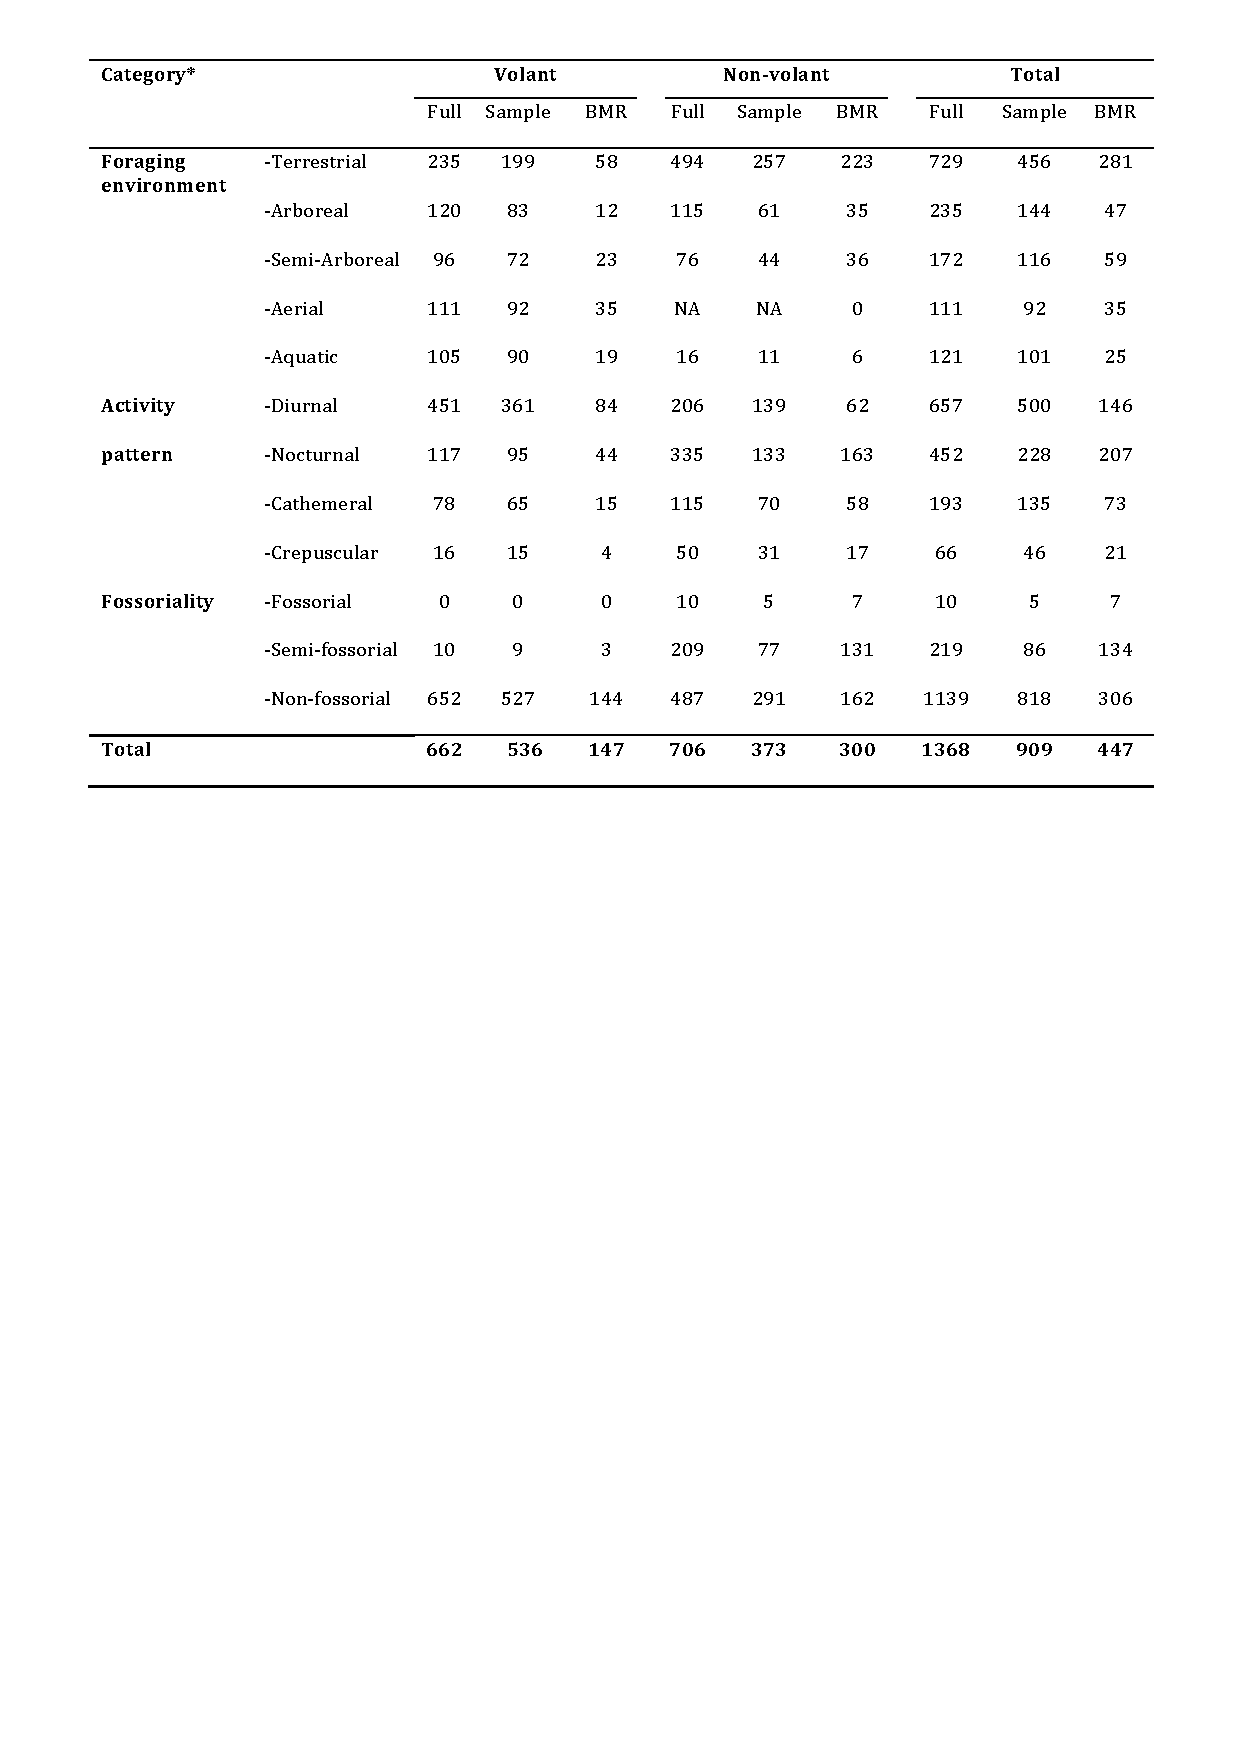
\includegraphics[width=\linewidth]{ch3-longevity-appendix/Table_B1.pdf}
\end{table}


\begin{table}[h]
  \caption[Table B2.]{Table B2: Relationship between maximum longevity (years), body mass (g) and flight capability (volant or non-volant) in 909 species of birds and mammals with over 100 maximum lifespan records.}
  \label{tbl:Table B2.}
  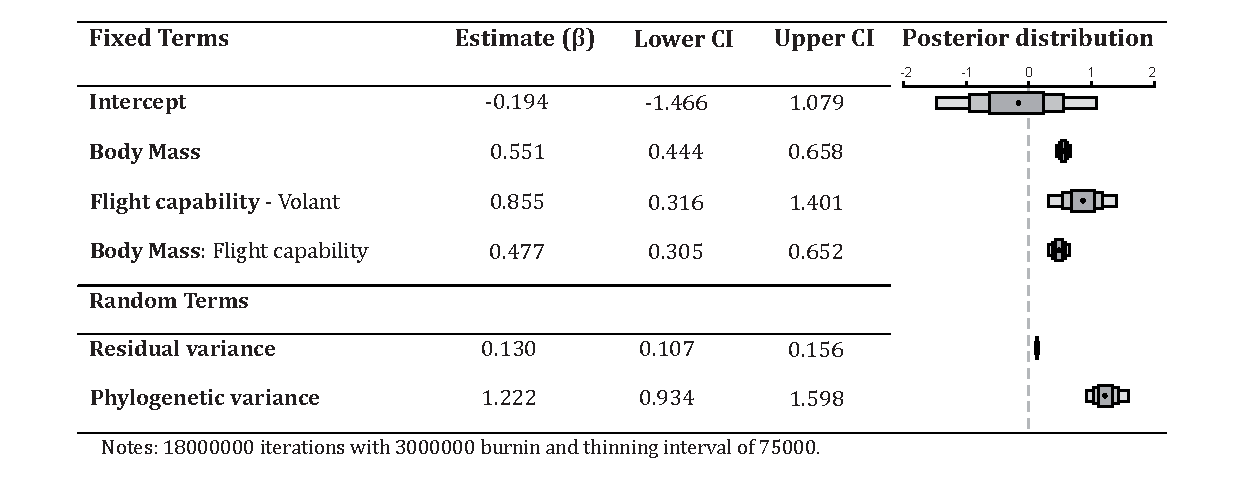
\includegraphics[width=\linewidth]{ch3-longevity-appendix/Table_B2.pdf}
\end{table}


\begin{table}[h]
  \caption[Table B3.]{Table B3: Relationship between maximum longevity (years), body mass (g), foraging environment and activity period, in 536 species of volant birds and mammals with over 100 samples of longevity.}
  \label{tbl:Table B3.}
  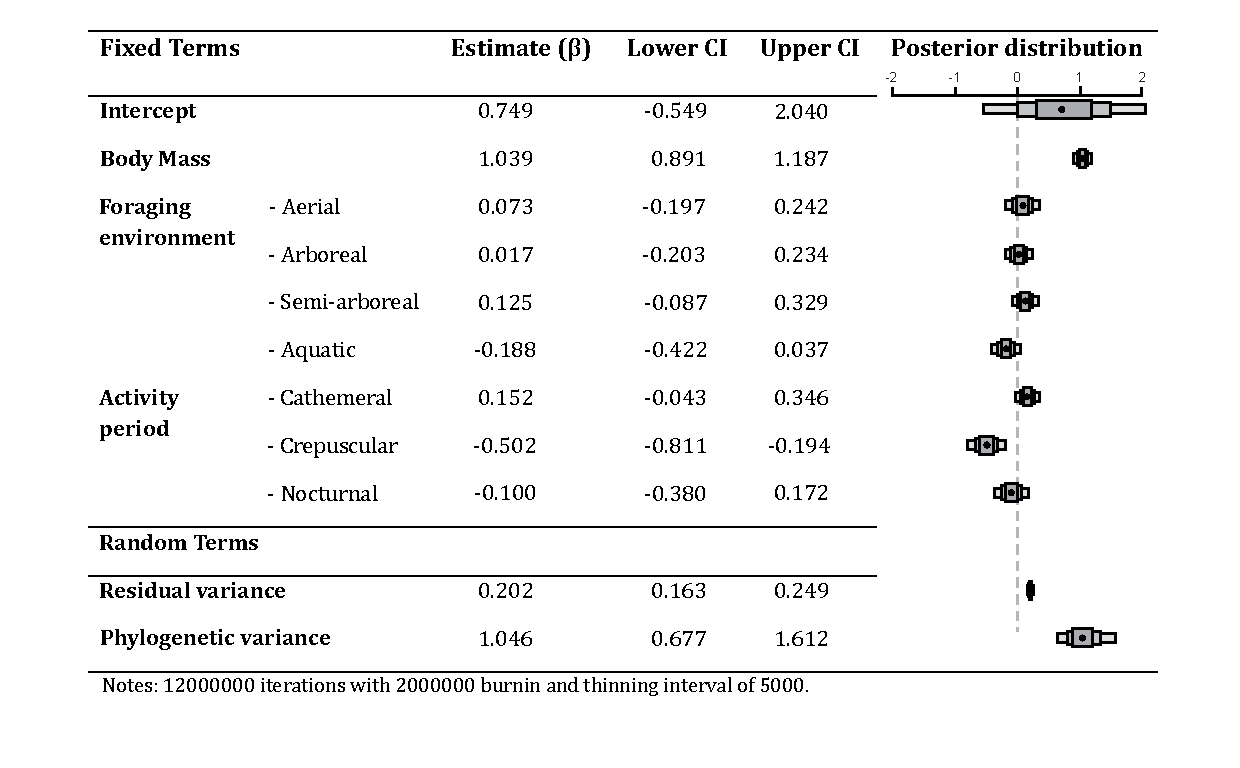
\includegraphics[width=\linewidth]{ch3-longevity-appendix/Table_B3.pdf}
\end{table}


\begin{table}[h]
  \caption[Table B4.]{Table B4: Relationship between maximum longevity (years), body mass (g), foraging environment, fossoriality and activity period, in 373 species of nonvolant birds and mammals with over 100 samples of longevity.}
  \label{tbl:Table B4.}
  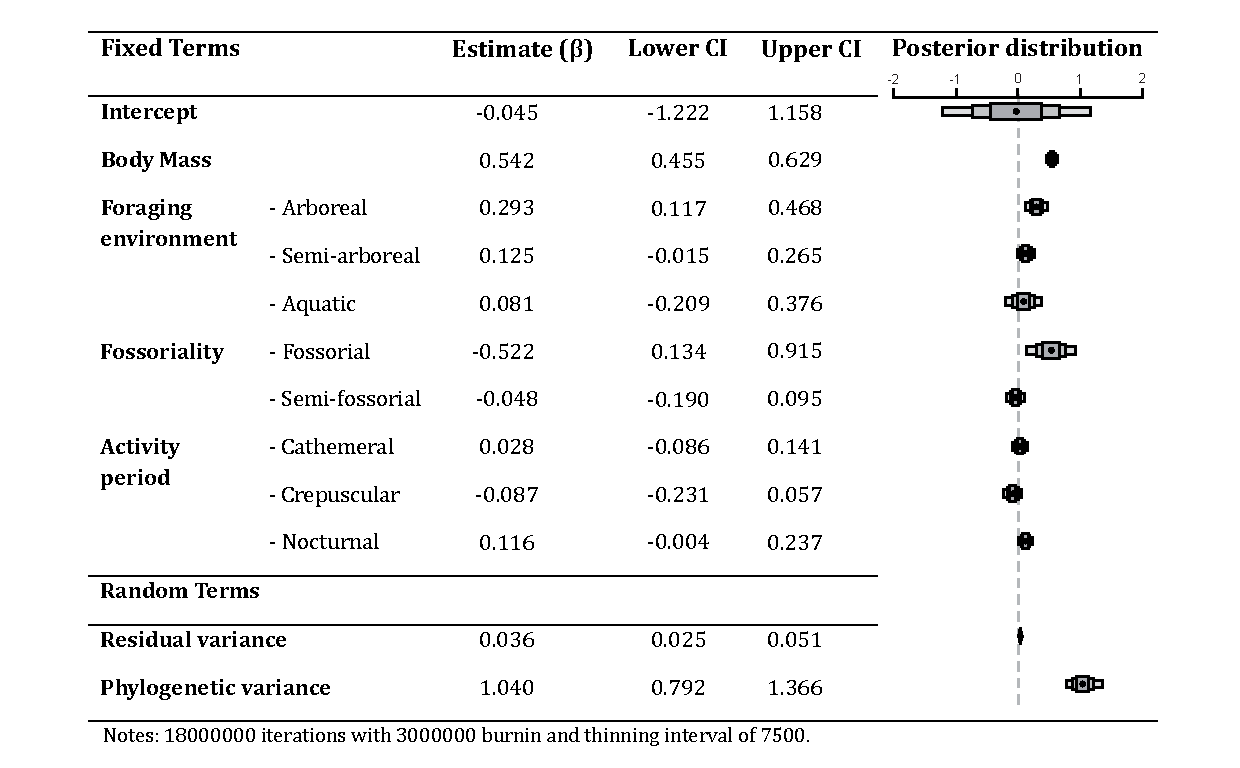
\includegraphics[width=\linewidth]{ch3-longevity-appendix/Table_B4.pdf}
\end{table}



\begin{table}[h]
  \caption[Table B5.]{Relationship between maximum longevity (years), body mass (g), foraging environment and activity period in 589 birds.}
  \label{tbl:Table B5.}
  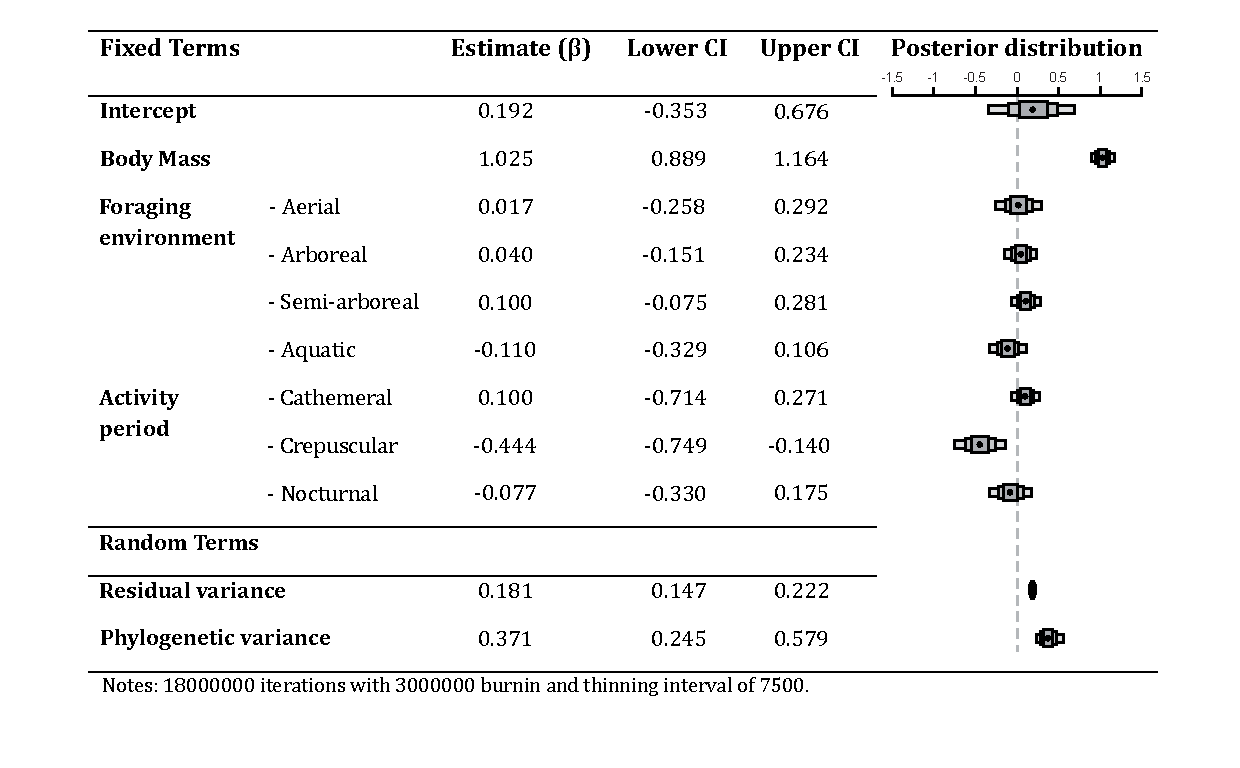
\includegraphics[width=\linewidth]{ch3-longevity-appendix/Table_B5.pdf}
\end{table}


\begin{table}[h]
  \caption[Table B6.]{Relationship between maximum longevity (years), body mass (g), foraging environment, fossoriality, and activity period 779 mammals..}
  \label{tbl:Table B9.}
  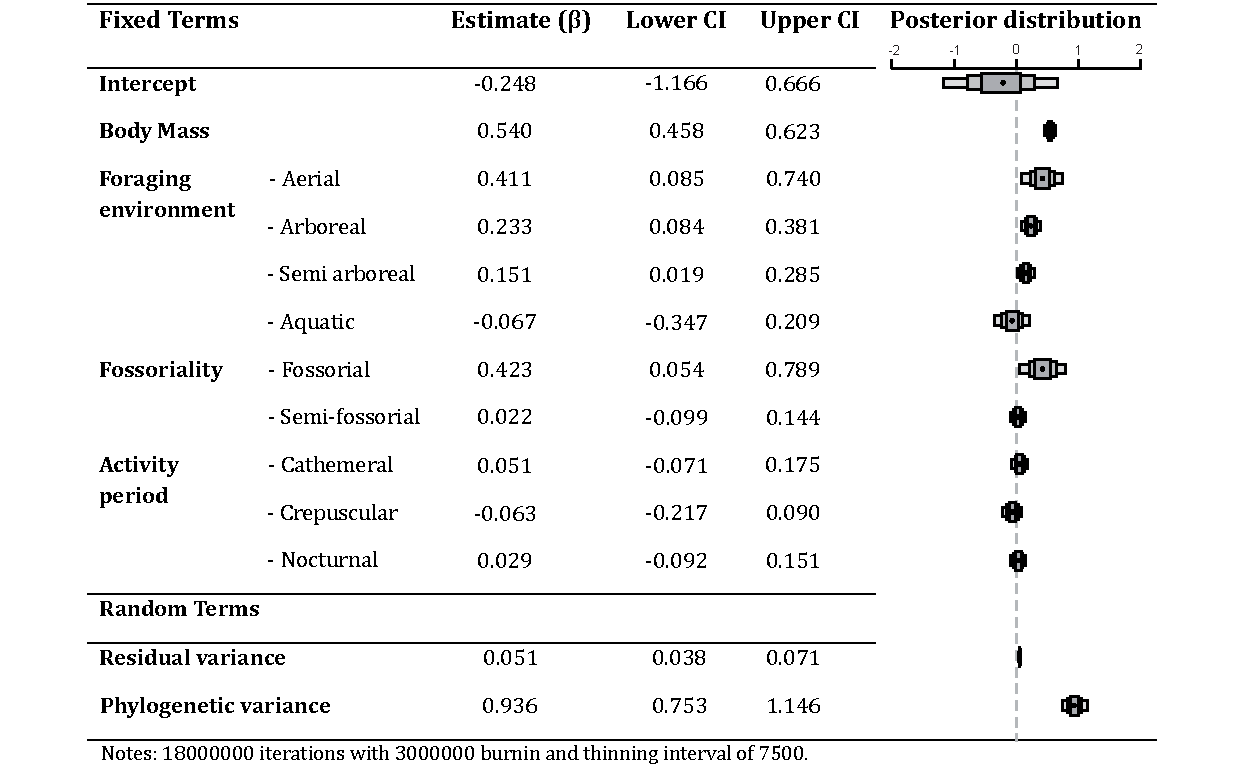
\includegraphics[width=\linewidth]{ch3-longevity-appendix/Table_B6.pdf}
\end{table}



\bibliographystyle{PLoS-Biology}
\bibliography{bibfile}




\end{document}
